\section{Methodology}
\label{thirdchapter}

%===============================================================
\subsection{Introduction}
%===============================================================
This chapter presents the methodology developed to evaluate and optimise composite steel--concrete floor slabs with respect to Global Warming Potential (GWP). The approach extends an existing parametric optimisation framework, originally developed by the Chair of Concrete Structures and Bridge Design at ETH Zurich for reinforced concrete and timber slab systems, to incorporate composite slab cross-sections. This extension enables the first systematic Eurocode-compliant comparison between conventional reinforced concrete flat slabs and composite slabs across a range of practical span lengths and occupancy scenarios. The methodology is implemented in Python and structured around a relational database of commercially available deck and concrete products, from which minimum-GWP cross-sections are identified for each span using a scalar bounded optimisation algorithm. The overall workflow, including the loop structure, the optimisation step, and the limit-state checks, is summarised in Figure~\ref{fig:code_flowchart}.

The chapter is structured as follows. Section~\ref{sec:prior_work} describes the pre-existing framework that this work extends. Section~\ref{sec:database} details the material and product database. Section~\ref{sec:casestudies} defines the case studies, including loading scenarios and floor build-ups. Section~\ref{sec:design_vars} sets out the design variables and design parameters. Section~\ref{sec:design_procedure} presents the structural verification procedure with the governing equations for each limit state, followed by the fire and acoustic design provisions. Section~\ref{sec:env_impact} outlines the environmental impact calculation. Section~\ref{sec:optimisation} describes the optimisation algorithm and convergence behaviour. Section~\ref{sec:validation} reports the validation against manufacturer design tables. Finally, Section~\ref{sec:assumptions} sets out the principal assumptions and limitations of the methodology.

%===============================================================
\subsection{Pre-existing framework}
\label{sec:prior_work}
%===============================================================
The composite slab module developed in this study is integrated into a pre-existing Python optimisation framework developed at the Chair of Concrete Structures and Bridge Design. The pre-existing framework provides cross-section classes for reinforced concrete rectangular slabs, reinforced concrete rib slabs, and several timber typologies (rectangular, box, and ribbed sections). For each typology, the framework performs ultimate limit state, serviceability limit state, and fire design checks in accordance with the relevant Eurocodes and Swiss standards, and quantifies GWP, cost (work in progress), and material quantities for use as objective functions in the optimisation.

The code is organised into two layers. The \textit{cross-section layer} (\texttt{struct\_analysis.py}) holds material and geometric properties for a given cross-section and evaluates section-level resistances and limit state checks. Each cross-section type (e.g.\ \texttt{RCSlab}, \texttt{TimberSlab}, \texttt{CompositeSlab}) is implemented as a class; instantiating it with a set of design parameters computes all relevant properties and runs the applicable checks. The \textit{member layer} (\texttt{struct\_optimization.py} and the per-configuration scripts) drives the optimisation: it iterates over spans, deck products, and concrete grades, instantiates cross-sections, and calls the optimiser to minimise the objective function (GWP) subject to structural feasibility. This separation means that structural logic is fully self-contained within each cross-section class and can be tested independently of the optimisation.

The pre-existing database is a SQLite file generated from an Excel workbook, organised into three tables: \texttt{material\_prop} (mechanical properties of concrete, reinforcing steel, and timber grades), \texttt{products} (Environmental Product Declaration data linked to material entries), and \texttt{floor\_struc\_prop} (non-structural floor build-up layer properties). The contribution of the present study to the database structure consists of an additional table, \texttt{sheeting\_prop}, containing the properties of profiled steel decking products required for composite slab design (described in Section~\ref{sec:database}), together with extensions to the \texttt{material\_prop} and \texttt{floor\_struc\_prop} tables to incorporate additional EPD entries and floor build-up layers relevant to composite construction.

The implementation in this study introduces a new \texttt{CompositeSlab} class within the cross-section module \texttt{struct\_analysis.py}, a corresponding optimisation routine \texttt{opt\_comp\_slab} within \texttt{struct\_optimization.py}, and member-level analysis scripts for simply-supported (\texttt{simple\allowbreak\_span\_composite.py}), two-span (\texttt{two\_span\_composite.py}), and three-span (\texttt{three\_span\_composite.py}) configurations, alongside auxiliary scripts for validation, end-anchorage comparison, GWP breakdown plotting, and vibration checking.

%===============================================================
\subsection{Material database}
\label{sec:database}
%===============================================================
The optimisation draws on the SQLite database described above. Of the four tables, the \texttt{sheeting\_prop} table is introduced as part of this study; the other three are inherited from the pre-existing framework with additional entries added to support composite slab design. The structure and contents of each table are described below.

\subsubsection*{Decking products (\texttt{sheeting\_prop})}
The decking table contains product-specific mechanical properties required for structural verification: rib geometry parameters $h_p$ (rib height), $l_1$ (rib pitch), $l_2$ (lower flange width), $l_3$ (upper flange width), sheet thickness $t$, web inclination $\theta$, and per-metre cross-sectional area $A_p$ and effective area $A_{p,e}$; section properties $e$ (centroidal axis from soffit), $e_p$ (effective centroidal axis), $I_p$ (second moment of area), $W_{pl}$ (plastic modulus), $W_{el,f}$ (effective elastic modulus); resistance values $M_{c,Rd}$ (sagging moment resistance), $M_{t,Rd}$ (hogging moment resistance, where available), and $f_{ypd}$ (design yield strength). Longitudinal shear parameters are stored where available, in one of two formats depending on the characterisation method adopted by the manufacturer: the m--k constants $(m_p, k_p)$ or the characteristic shear bond strength $\tau_{u,Rk}$ from EN~1994-1-1 Cl.\,9.7.3.

The volume of concrete that fills the trough voids is stored as the parameter $V_\mathrm{tr}$ (in m$^3$/m$^2$), derived from the manufacturer-declared concrete volume per square metre and used in the GWP and self-weight calculations as described in Section~\ref{sec:env_impact}.

Environmental data are stored as a GWP value accompanied by a unit descriptor (\texttt{GWP\_UNIT}), since manufacturer EPDs express results in differing functional units---per unit area (kg\,CO$_2$-eq/m$^2$) or per unit mass (kg\,CO$_2$-eq/t)---and normalisation to a consistent per-metre-length basis is applied within the model.

Deck products currently included in the database are drawn from the ComFlor range produced by Tata Steel, the Cofraplus and Cofradal ranges from ArcelorMittal, and the Multideck range from Kingspan. These manufacturers were selected on the basis of EPD and property availability, coverage of both shallow ($h_p \le 80$\,mm) and deep ($h_p \ge 200$\,mm) decking profiles, and suitability for the span range under investigation, as discussed in Section~\ref{sec:commercial_slim_floor}.

Mechanical property data was obtained from the manufacturer technical manuals \citep{RefWorks:2017comflor, RefWorks:2021floors, RefWorks:kingspan2026multideck} as well as the manufacturers' design software (ComFlor analysis software, COFRA 5 and Kingspan Catalyst respectively), and EPD values were sourced from the corresponding manufacturer-published declarations. 

\subsubsection*{Material properties (\texttt{material\_prop})}
The material property table contains design properties for concrete, timber, and steel: characteristic compressive strength $f_{ck}$, mean tensile strength $f_{ctm}$, mean elastic modulus $E_{cm}$, dry and wet unit weights, and (for reinforcement) characteristic yield strength $f_{sk}$, modulus $E_s$, cross-sectional area per metre $A_s$, and bar diameter $d_s$. For mesh reinforcement, standard fabric types A142, A193, A252, and A393 are listed (per BS~4483:2025). For timber, additional properties such as bending and shear strengths and burn rate are included.

\subsubsection*{Products (\texttt{products})}
The products table is the environmental data library of the framework, inherited from the prior work and extended for this study. Each row holds an Environmental Product Declaration (EPD) entry, or an equivalent life-cycle dataset, for a structural or non-structural material, linked to a mechanical-property entry through the \texttt{MECH\_PROP} key. The table spans the material families used across the framework's slab typologies---ready-mixed concrete, reinforcing steel, structural steel sections, prestressing steel, and engineered timber (glue-laminated, cross-laminated, and solid timber).

For each entry the table records the Global Warming Potential together with metadata establishing its provenance and validity: the data \emph{source}, the EPD identifier with its issue and expiry dates, the country of declaration, the declared density and (for concrete) the cement type and exposure class, and cross-reference identifiers to the KBOB and Ökobaudat catalogues. The GWP is stored not as a single figure but split into life-cycle stages---modules A1--A3 (cradle-to-gate) and C1--C4 (end-of-life)---so that the system boundary adopted in Section~\ref{sec:env_impact} can be assembled consistently from the same underlying data. Flags record whether an entry is a verified EPD and whether it remains within its validity period.

The entries are drawn from many sources, ranging from product-specific to generic:
\begin{itemize}
    \item \textbf{Manufacturer and industry-association EPDs}---verified, product-specific declarations to EN~15804 / ISO~14025. For concrete these include sector EPDs published by the Swiss concrete association (FSKB) for the standard Swiss concrete sorts (NPK~A--G); for reinforcing steel they include producer EPDs from a range of European mills.
    \item \textbf{ecoinvent}---the generic background life-cycle inventory database \citep{RefWorks:ecoinvent2024}, used for Swiss ready-mixed concrete mixes where no product-specific EPD is available. ecoinvent also supplies the background process data underlying the FSKB sector EPDs and the \emph{Betonsortenrechner} concrete-mix calculator entries.
    \item \textbf{KBOB}---the reference dataset \emph{Ökobilanzdaten im Baubereich} \citep{RefWorks:kbob2022} (version~7), published by the Swiss coordination group of public-sector building owners. KBOB provides representative, averaged GWP intensities for common construction materials and is the de-facto reference for embodied-carbon assessment in Swiss practice.
\end{itemize}

The KBOB dataset serves three distinct roles in this study: it provides the GWP intensities for the non-structural floor build-up layers (Section~\ref{sec:floor_buildup}); it provides the representative concrete and reinforcement intensities used for the reinforced-concrete baseline, consistent with the prior framework; and it acts as the independent benchmark against which the manufacturer steel-decking EPDs were assessed, motivating the exclusion of the ArcelorMittal data discussed in Section~\ref{sec:assumptions}.

The GWP of mesh reinforcement is not stored separately in the products table; instead, the GWP per unit mass of B500B reinforcing steel is applied as a representative value, consistent with the treatment of reinforcement in the reinforced-concrete baseline model.

\subsubsection*{Floor build-up (\texttt{floor\_struc\_prop})}
Non-structural floor build-up layers are listed with their height, density, weight, and GWP per unit mass; the per-layer GWP intensities are taken from the KBOB dataset \citep{RefWorks:kbob2022}. The layers used in this study are described in Section~\ref{sec:floor_buildup}. The permanent load contribution of the floor build-up to the composite slab design ($g_{k,\mathrm{fin}}$) is derived directly from the summed self-weight of the declared layers in the database (\texttt{FloorStruc.gk\_area}, in N/m$^2$), ensuring consistency between the GWP calculation and the structural loading used in the optimisation.

%===============================================================
\subsection{Case studies and loading scenarios}
\label{sec:casestudies}
%===============================================================
\subsubsection*{Loading scenarios}

Four occupancy scenarios are evaluated, corresponding to typical multi-storey applications of composite floor systems: \textbf{office}, \textbf{residential}, \textbf{retail}, and \textbf{industrial}. For each scenario, the imposed load $q_k$ and the partition allowance $q_{k,\mathrm{part}}$ are taken from 1-1-1 Table~6.2 according to the use category. The permanent service load $g_{k,\mathrm{serv}}$ represents a fixed services and fittings allowance above the structural slab. Loading parameters for each scenario are summarised in Table~\ref{tab:loading_scenarios}.

\begin{table}[h!]
\small
\centering
\caption{Loading parameters per occupancy scenario.}
\label{tab:loading_scenarios}
\begin{tabular}{lcccccc}
\toprule
Scenario & Cat. & $q_k$ & $q_{k,\mathrm{part}}$ & $g_{k,\mathrm{serv}}$ & $Q_{k,\mathrm{constr}}$ & $\psi_\mathrm{fi}$ \\
         &      & [kN/m$^2$] & [kN/m$^2$] & [kN/m$^2$] & [kN/m$^2$] & [--] \\
\midrule
Residential & A  & 2.0 & ---  & 0.75 & 0.75 & 0.5 \\
Office      & B  & 2.5 & 0.50 & 0.75 & 0.75 & 0.5 \\
Retail      & D1 & 4.0 & ---  & 0.50 & 0.75 & 0.7 \\
Industrial  & E1 & 7.5 & ---  & 0.50 & 0.75 & 0.9 \\
\bottomrule
\end{tabular}
\end{table}

The construction-stage imposed load follows 1-1-6/4.11.2: a uniformly distributed load $Q_{k,1b} = 0.75$\,kN/m$^2$ representing personnel and small equipment is applied across the full span, with an additional $0.75$\,kN/m$^2$ patch load applied over a $3 \times 3$\,m working area (giving a total patch load of $1.5$\,kN/m$^2$) to represent localised concentrations of workers and equipment during pouring. The wet concrete weight $Q_{k,1c}$ is computed from the wet density of the chosen concrete grade and the average concrete depth $h_\mathrm{c,avg}$ (defined in Section~\ref{sec:env_impact}). A minimum base uniform load $Q_{k,1a} = \max(0.75,\;0.10\,Q_{k,1c})$\,kN/m$^2$ is also defined, representing the case where the concrete is heavier than the nominal construction load, to ensure that the construction stage is never under-designed relative to the actual wet concrete weight.

\subsubsection*{Floor build-up}
\label{sec:floor_buildup}

The floor build-up above the structural slab is selected for each occupancy scenario to satisfy the relevant acoustic requirements while minimising additional GWP. The acoustic requirements are taken from SIA~181 \citep{RefWorks:sia181} for the Swiss context and cross-checked against Approved Document E \citep{RefWorks:adePartE} for the UK context, as discussed in Section~\ref{sec:acoustic}. The build-up layers used in this study are listed in Table~\ref{tab:floor_buildup} and shown schematically in Figure~\ref{fig:floor_buildups}.

\begin{figure}[h!]
  \centering
  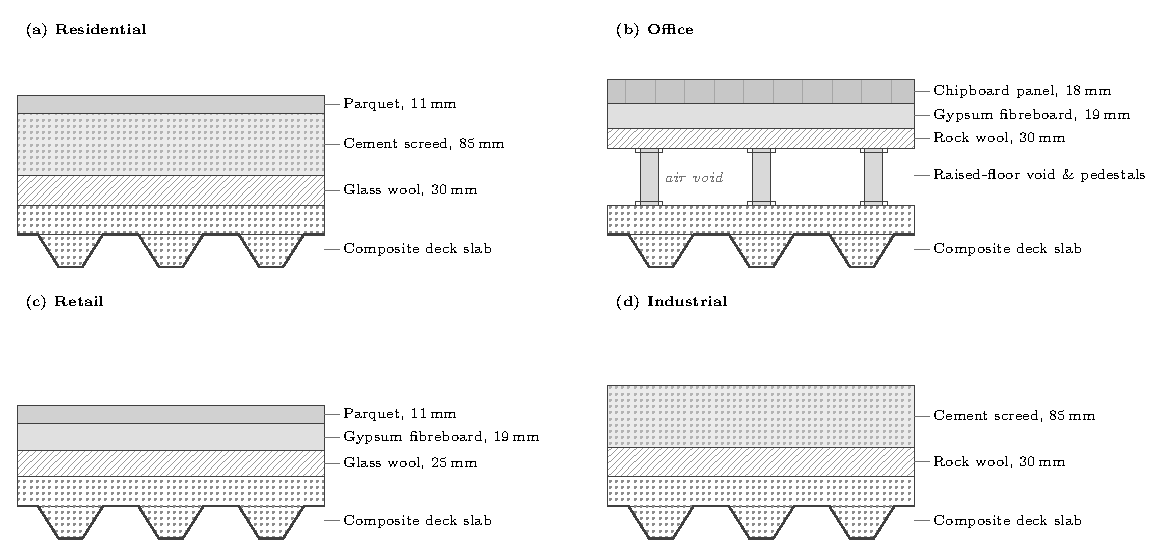
\includegraphics[width=\textwidth]{figures/floor_buildups.pdf}
  \caption{Schematic cross-sections of the floor build-up adopted for each occupancy scenario, shown above the composite steel deck slab. Vertical proportions are exaggerated for clarity and are not to scale. Hatching denotes material type: dotted for cementitious layers (screed and concrete), diagonal for mineral-wool insulation, and solid grey for boards and parquet finishes.}
  \label{fig:floor_buildups}
\end{figure}

\begin{table}[h!]
\small
  \centering
  \caption{Floor build-up layers per occupancy scenario (top to bottom, above structural slab).}
  \label{tab:floor_buildup}
  \begin{tabular}{llccc}
    \toprule
    Scenario & Layer (top to bottom) & Thickness [mm] & Density [kg/m\textsuperscript{3}] & GWP [kg\,CO\textsubscript{2}/kg] \\
    \midrule
    \multirow{3}{*}{Residential}
      & 2-layer factory-sealed parquet & 11 & 555  & 1.28 \\
      & Cement screed                  & 85 & 1850 & 0.12 \\
      & Glass wool insulation          & 30 & 80   & 1.10 \\
    \cmidrule(lr){1-5}
    \multirow{3}{*}{Office}
      & Chipboard panel       & 18 & 640  & 0.53 \\
      & Gypsum fibreboard     & 19 & 1200 & 0.55 \\
      & Rock wool insulation  & 30 & 38   & 0.82 \\
    \cmidrule(lr){1-5}
    \multirow{3}{*}{Retail}
      & 2-layer factory-sealed parquet & 11 & 555  & 1.28 \\
      & Gypsum fibreboard              & 19 & 1200 & 0.55 \\
      & Glass wool insulation          & 25 & 80   & 1.10 \\
    \cmidrule(lr){1-5}
    \multirow{2}{*}{Industrial}
      & Cement screed        & 85 & 1850 & 0.12 \\
      & Rock wool insulation & 30 & 38   & 0.82 \\
    \bottomrule
  \end{tabular}
\end{table}

\subsubsection*{Span ranges and configurations}
The slab is evaluated as a one-way spanning system across spans of 3--10\,m in 1\,m increments, encompassing the practical range for both shallow ($h_p \le 80$\,mm) and deep ($h_p \ge 200$\,mm) decking profiles. Three span configurations are evaluated for each loading scenario:
\begin{itemize}
    \item Single span (simply supported)
    \item Two-span continuous
    \item Three-span continuous
\end{itemize}
Multi-span configurations use equal spans throughout; the influence of unequal spans is not investigated. All structural verification and optimisation is carried out on a per-metre-width basis, allowing results to be expressed as GWP per metre of span length in kg\,CO$_2$-eq/m.

%===============================================================
\subsection{Design variables and parameters}
\label{sec:design_vars}
%===============================================================
The optimisation considers three categories of design variable, summarised in Table~\ref{tab:opt_variables}. The single continuous variable $h$ is optimised by the bounded scalar algorithm; discrete variables are enumerated in an outer loop over all admissible options.

\begin{table}[h!]
\small
\centering
\caption{Optimisation variables and their treatment}
\label{tab:opt_variables}
\begin{tabular}{p{5cm} p{2.5cm} p{2cm} p{4cm}}
\toprule
\textbf{Variable} & \textbf{Symbol} & \textbf{Type} & \textbf{Range / set} \\
\midrule
Total slab depth                  & $h$            & Continuous & $h_p + 50$\,mm $\le h \le 500$\,mm \\
Steel deck product                & ---            & Discrete (enum.) & All products in \texttt{sheeting\_prop} \\
Concrete grade                    & $f_{ck}$       & Discrete (enum.) & C25/30, C30/37 \\
Mesh reinforcement                & $A_s$          & Discrete (auto-selected) & A142, A193, A252, A393 \\
Trough bar diameter (fire only)   & $\varnothing_\mathrm{tr}$ & Discrete (auto-selected) & 8, 10, 12, 16, 20\,mm \\
\bottomrule
\end{tabular}
\end{table}

The minimum permissible total depth is the deck rib height $h_p$ plus a minimum concrete cover of 50\,mm above the top of the ribs, in accordance with 4-1-1/9.2.1, and not less than 90\,mm. The upper search bound is 500\,mm, accommodating the deepest deck profiles at long spans. Both propped and unpropped construction are evaluated: the optimiser first attempts unpropped construction; if no feasible solution exists within the search bounds, a second pass with propped construction is performed.

The mesh reinforcement is selected automatically as the lightest fabric type satisfying the minimum longitudinal reinforcement ratio of 4-1-1/9.8.1, namely $0.2\%\,A_c$ for unpropped construction (or $0.4\%\,A_c$ if propped). The hogging ULS check at internal supports (Section~\ref{sec:hogging}) and the fire D2/D3 checks (Section~\ref{sec:fire}) may upgrade the mesh to a heavier fabric if required.

Trough bar reinforcement within the deck ribs is not considered for structural ULS checks. The fire design procedure (Section~\ref{sec:fire}) selects the minimum trough bar diameter required for the sagging moment check at elevated temperature; if no diameter from the available set produces a passing fire check, the cross-section is recorded as failing the D2 check.

Table~\ref{tab:design_parameters} summarises the design parameters held constant across all configurations. All quantities in the \texttt{material\_prop} and \texttt{floor\_struc\_prop} tables follow the SI convention adopted throughout this tool (N, m). The \texttt{sheeting\_prop} table follows the engineering convention standard in EN 1994-1-1 and manufacturer datasheets: geometric dimensions in mm, second moments of area in cm$^4$/m, cross-sectional areas in mm$^2$/m, strength values in N/mm$^2$, and moment capacities in kNm/m. Internally, the \texttt{CompositeSlab} class converts between these conventions at the point of use.

\begin{table}[h!]
\scriptsize
\centering
\caption{Summary of design parameters, loading assumptions, and partial factors}
\label{tab:design_parameters}
\renewcommand{\arraystretch}{1.3}
\begin{tabular}{p{6.5cm} p{1.8cm} p{2.8cm} p{3.0cm}}
\hline
\textbf{Parameter} & \textbf{Symbol} & \textbf{Value / Assumption} & \textbf{Reference} \\
\hline
\multicolumn{4}{l}{\textit{Construction-stage Loads}} \\
\hline
Construction stage UDL          & $Q_{k,1b}$        & 0.75 kN/m²         & EN 1991-1-6 Cl.\,4.11.2 \\
Construction stage patch load   & $Q_{k,1b,\mathrm{patch}}$ & 1.5 kN/m² over 3$\times$3 m & EN 1991-1-6 Cl.\,4.11.2 \\
\hline
\multicolumn{4}{l}{\textit{Partial Factors}} \\
\hline
Permanent loads                 & $\gamma_G$        & 1.35               & EN 1990 \\
Variable loads                  & $\gamma_Q$        & 1.50               & EN 1990 \\
Concrete                        & $\gamma_C$        & 1.50               & EN 1992-1-1 \\
Reinforcement                   & $\gamma_S$        & 1.15               & EN 1992-1-1 \\
Steel section                   & $\gamma_{M0}$     & 1.00               & EN 1993-1-1 \\
Longitudinal shear              & $\gamma_{VS}$     & 1.25               & EN 1994-1-1 Cl.\,9.7.3 \\
\hline
\multicolumn{4}{l}{\textit{Serviceability Limits}} \\
\hline
Construction stage deflection   & $\delta_\mathrm{constr}$  & $\min(L/180, 20\,\mathrm{mm})$ or $\min(L/130, 30\,\mathrm{mm})$    & EN 1994-1-1 Cl.\,9.3.2; UK NA \\
Composite stage --- total       & $\delta_\mathrm{tot}$     & $L/300$                            & SIA 263$^{\ddagger}$ \\
Composite stage --- variable    & $\delta_\mathrm{var}$     & $\min(L/350, 20\,\mathrm{mm})$    & EN 1994-1-1 Cl.\,9.8.2(4) \\
\hline
\multicolumn{4}{l}{\textit{Cross-section Constraints}} \\
\hline
Minimum concrete cover above deck & ---             & 50\,mm                            & EN 1994-1-1 Cl.\,9.2.1 \\
Minimum total depth              & ---             & $h_p + 50$\,mm; not less than 90\,mm & EN 1994-1-1 Cl.\,9.2.1 \\
Concrete cover to top mesh       & $c_\mathrm{nom}$ & 20\,mm                            & EN 1992-1-1 Cl.\,4.4 \\
\hline
\multicolumn{4}{l}{\textit{Material Properties}} \\
\hline
Effective deck area (where not stated) & $A_{p,e}$ & $0.9\,A_p$ (shallow); $0.5\,A_p$ (deep, $h_p \ge 80$\,mm) & $^{\dagger}$ \\
Creep coefficient                & $\varphi_t$    & EN 1992-1-1 Annex B & EN 1992-1-1 Cl.\,5.4.2.2 \\
Modular ratio (short-term)       & $n_0$          & $E_a / E_{cm}$ & EN 1994-1-1 Cl.\,5.4.2.2 \\
Modular ratio (long-term)        & $n_L$          & $n_0(1 + 1.1\varphi_t)$ & EN 1994-1-1 Cl.\,5.4.2.2 \\
Cement class                     & ---            & N (normal)              & EN 1992-1-1 \\
Relative humidity                & RH             & 50\% (interior)         & EN 1992-1-1 Annex B \\
Loading age                      & $t_0$          & 28 days                 & SCI P359 Cl.\,6.3 \\
\hline
\multicolumn{4}{l}{\textit{Fire Design}} \\
\hline
Fire resistance period           & $R_\mathrm{fi}$    & R60 & EN 1994-1-2 Annex D \\
Fire combination factor          & $\psi_\mathrm{fi}$ & 0.5 -- 0.9 (occupancy-dependent)        & EN 1990 Table A1.1 \\
Trough bar diameter set          & $\varnothing_\mathrm{tr}$ & $\{8, 10, 12, 16, 20\}$\,mm    & --- \\
\hline
\multicolumn{4}{l}{\textit{Environmental Assessment}} \\
\hline
LCA system boundary              & ---            & A1--A3 and C1--C4              & EN 15804 \\
Functional unit                  & ---            & kg\,CO$_2$-eq/m of span length & --- \\
\hline
\end{tabular}
\vspace{4pt}\\
{\footnotesize
$^{\ddagger}$ EN~1994-1-1 Cl.\,9.8.2(4) recommends a total deflection limit of $L/250$; the more conservative limit of $L/300$ is adopted here in accordance with SIA~263 \citep{RefWorks:sia263}, for consistency with the prior framework against which the composite results are compared.\\
$^{\dagger}$ Conservative fallback: $A_{p,e} = 0.9\,A_p$ for shallow profiles ($h_p < 80$\,mm); $A_{p,e} = 0.5\,A_p$ for deep profiles ($h_p \ge 80$\,mm). Where the manufacturer publishes $A_{p,e}$ explicitly it is used directly.
}
\end{table}

%===============================================================
\subsection{Design procedure}
\label{sec:design_procedure}
%===============================================================
Structural verification follows the staged nature of composite construction, distinguishing between the \textbf{construction stage}, in which the concrete is wet and only the steel deck resists loads, and the \textbf{composite stage}, in which the hardened concrete and the deck act together. Checks are performed in accordance with EN~1994-1-1/2 supplemented by EN~1992-1-1 and EN~1993-1-3. The full set of checks evaluated by the model is listed in Table~\ref{tab:checks_summary}.

\begin{table}[h!]
\small
\centering
\caption{Limit state checks performed by the composite slab module}
\label{tab:checks_summary}
\begin{tabular}{p{2.5cm} p{4.0cm} p{6.5cm}}
\toprule
\textbf{Stage} & \textbf{Check} & \textbf{Reference} \\
\midrule
Construction$^{\dagger}$ & ULS bending (sagging) & EN 1993-1-3 Cl.\,5.4.3, EN 1994-1-1 Cl.\,9.3 \\
Construction$^{\dagger}$ & ULS web shear buckling      & EN 1993-1-3 Cl.\,6.1.5 \\
Construction$^{\dagger}$ & SLS deflection              & EN 1994-1-1 Cl.\,9.3.2; UK NA \\
Composite    & ULS sagging moment          & EN 1994-1-1 Cl.\,9.7.2 \\
Composite    & ULS longitudinal shear      & EN 1994-1-1 Cl.\,9.7.3 (m--k) or 9.7.5 ($\tau_u$) \\
Composite    & ULS vertical shear          & EN 1994-1-1 Cl.\,9.7.5; EN 1992-1-1 Cl.\,6.2.2 (2004)\\
Composite    & ULS hogging (cont.\ spans)  & EN 1994-1-1 Cl.\,9.7.3(2)P, 9.4.2(3) \\
Composite    & SLS deflection (total \& variable) & SIA 263; EN 1994-1-1 Cl.\,9.8.2(4) \\
Fire         & D1: thermal insulation      & EN 1994-1-2 Annex D, formula D.1 \\
Fire         & D2: sagging moment $M_\mathrm{Rd,fi}$ & EN 1994-1-2 Annex D, formulae D.4--D.5 \\
Fire         & D3: hogging $M_\mathrm{Rd,fi}$ (cont.) & EN 1994-1-2 Annex D, formulae D.7--D.11 \\
Fire         & D4: minimum effective thickness & EN 1994-1-2 Annex D, Table D.6 \\
Fire         & D5: field of application    & EN 1994-1-2 Annex D, Table D.7 \\
\bottomrule
\end{tabular}
\vspace{2pt}\\
{\footnotesize $^{\dagger}$ For propped construction, a single prop at midspan divides the span into two simply-supported $L/2$ sub-spans during casting (EN~1994-1-1 Cl.\,9.3.1); the construction-stage checks are therefore performed against the $L/2$ sub-span rather than omitted.}
\end{table}

\subsubsection*{Construction stage}
\label{sec:constr_stage}
During unpropped construction the profiled steel deck acts as temporary formwork and must resist the self-weight of the wet concrete, its own self-weight, and the construction imposed loads over the full distance between permanent supports. When propped construction is specified, a single temporary prop is assumed at midspan during casting, dividing each span into two simply-supported $L/2$ sub-spans. The deck still carries the full wet-concrete and construction loads, but over the reduced sub-span $L/2$; the construction-stage checks are therefore not omitted but are evaluated against the $L/2$ sub-span using simply-supported coefficients. Because the propped sub-spans are simply supported, no hogging develops at the permanent internal supports during casting, so the construction-stage hogging and internal-support checks are suppressed for the propped case. The reduced effective span is what makes propped construction feasible at longer spans, where the bare deck could not span the full distance unpropped.

\paragraph{ULS bending.} The construction-stage load model is shown in Figure~\ref{fig:constr_load_model}. The deck is verified against the maximum sagging moment $M_{Ed,sag}$, computed as the more onerous of two construction load cases:
\begin{align}
    M_{Ed,sag,1} &= \alpha_M \cdot w_\mathrm{ULS,1} \cdot L^2
    \label{eq:constr_sag_1} \\
    M_{Ed,sag,2} &= \alpha_M \cdot w_\mathrm{base} \cdot L^2 + M_\mathrm{patch}(q_\mathrm{patch}, a_\mathrm{patch}, L)
    \label{eq:constr_sag_2}
\end{align}
where $w_\mathrm{ULS,1} = \gamma_G G_{k,1a} + \gamma_Q (Q_{k,1a} + Q_{k,1b} + Q_{k,1c})$ combines all construction loads as a full-span UDL, $w_\mathrm{base} = \gamma_G G_{k,1a} + \gamma_Q (Q_{k,1b} + Q_{k,1c})$ is the base UDL excluding the patch enhancement, $q_\mathrm{patch} = \gamma_Q Q_{k,1a}$ is the factored patch load intensity, $a_\mathrm{patch} = 3$\,m, and $M_\mathrm{patch}$ is the mid-span moment contribution from the symmetrically placed patch load. The deck is treated as simply supported at the construction stage, so the sagging coefficient is $\alpha_M = 1/8$ in all cases. For multi-span configurations the deck is assumed to be lapped and effectively pinned over the permanent supports during casting (consistent with the SS treatment in SCI~P300); no continuity moment is taken at this stage. For propped construction the same $\alpha_M = 1/8$ applies, but to the $L/2$ sub-span between the prop and the permanent support (Section~\ref{sec:constr_stage}).

The sagging check is $M_{Ed,sag} \le M_{c,Rd}$, where $M_{c,Rd}$ is the manufacturer-published characteristic sagging moment resistance of the deck. Because the deck is treated as simply supported during casting, no construction-stage hogging check or moment redistribution is performed; the hogging resistance $M_{t,Rd}$ is used only for the composite-stage and fire hogging checks at internal supports (Sections~\ref{sec:hogging} and~\ref{sec:fire}).

\paragraph{ULS shear (web buckling).} Web shear buckling resistance per web is computed in accordance with EN~1993-1-3 Cl.\,6.1.5:
\begin{equation}
    V_{b,Rd,\mathrm{web}} = \frac{h_w \cdot t \cdot f_{bv}}{\sin\theta \cdot \gamma_{M0}}
    \label{eq:web_shear}
\end{equation}
where $h_w = h_p - t$ is the web height, $\theta$ is the web inclination, and $f_{bv}$ is the shear buckling strength obtained from the relative web slenderness $\bar{\lambda}_w = 0.346 \cdot s_w / t \cdot \sqrt{f_{ypd}/E}$:
\begin{equation}
    f_{bv} =
    \begin{cases}
    0.58\,f_{ypd} & \text{if } \bar{\lambda}_w \le 0.83 \\
    0.48\,f_{ypd}/\bar{\lambda}_w & \text{if } 0.83 < \bar{\lambda}_w < 1.40 \\
    0.67\,f_{ypd}/\bar{\lambda}_w^2 & \text{if } \bar{\lambda}_w \ge 1.40
    \end{cases}
    \label{eq:fbv}
\end{equation}
The total resistance is $V_{b,Rd} = N_w \cdot V_{b,Rd,\mathrm{web}}$, where $N_w$ is the number of webs per metre width, taken from the database. The design shear force is the more onerous of the two load-case resultants evaluated at the support.

\paragraph{SLS deflection.} The construction-stage SLS deflection check uses the initial elastic deflection of the bare deck under self-weight $G_{k,1a}$ and wet concrete weight $Q_{k,1c}$ only; construction live loads are excluded per EN~1994-1-1 Cl.\,9.3.2(2):
\begin{equation}
    \delta_\mathrm{initial} = K_\delta \cdot \frac{w_\mathrm{SLS} \cdot L^4}{E \cdot I_p}
    \label{eq:constr_defl}
\end{equation}
with $w_\mathrm{SLS} = G_{k,1a} + Q_{k,1c}$ (characteristic loads) and deflection coefficients $K_\delta = 5/384$ (single span), $2/369$ (two spans), $1/145$ (three or more spans). 

The deflection limit is selected based on whether ponding is significant, following the UK National Annex to EN~1994-1-1:
\begin{equation}
    \delta_\mathrm{limit} =
    \begin{cases}
    \min(L/180,\;20\,\mathrm{mm}) & \text{if } \delta_\mathrm{initial} \le h/10 \quad \text{(Option 1, no ponding)} \\
    \min(L/130,\;30\,\mathrm{mm}) & \text{if } \delta_\mathrm{initial} > h/10 \quad \text{(Option 2, ponding included)}
    \end{cases}
    \label{eq:constr_defl_limit}
\end{equation}
where $h$ is the total slab depth. When Option~2 applies ($\delta_\mathrm{initial} > h/10$), a ponding correction is applied: an extra wet-concrete UDL proportional to the current depression is added, and the resulting increased concrete volume is carried through to the GWP and self-weight calculations.

\begin{figure}[h!]
  \centering
  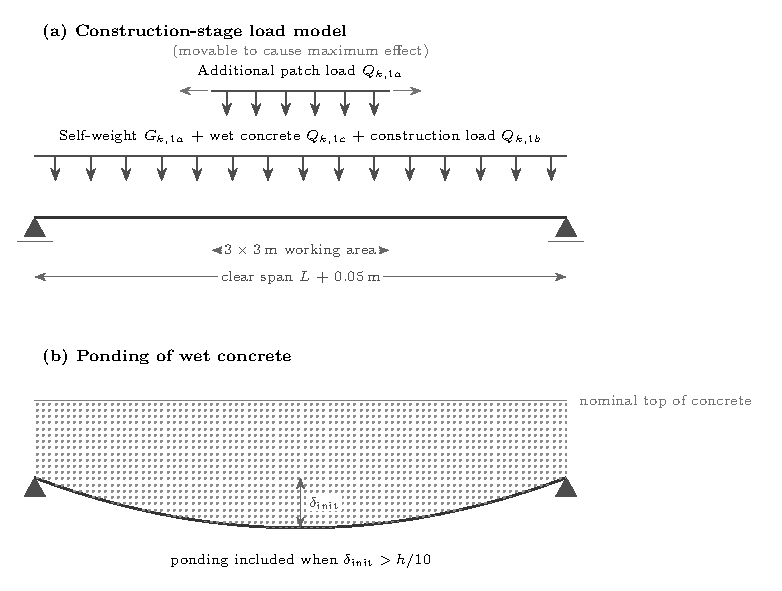
\includegraphics[width=0.9\textwidth]{figures/constr_load_model.pdf}
  \caption[Construction-stage load model]{Construction-stage load model on the profiled steel deck.}
  \label{fig:constr_load_model}
\end{figure}

\subsubsection*{Composite stage}
\label{sec:comp_stage}
Once the concrete has hardened, the slab and the deck act compositely through longitudinal shear transfer at the steel--concrete interface. Composite-stage checks apply to both propped and unpropped construction.

\paragraph{ULS sagging moment.} The composite sagging moment resistance assumes full shear connection and is calculated from a rectangular plastic stress block. The compression force in the concrete is governed by the lesser of the steel deck and concrete capacities:
\begin{equation}
    N_{cf} = \min\!\left(A_{p,e}\,f_{ypd},\; 0.85\,f_{cd}\,b\,h_c\right)
    \label{eq:Ncf}
\end{equation}
The depth of the rectangular concrete compression block is $x_{pl} = N_{cf}/(0.85\,f_{cd}\,b)$, and the plastic sagging moment resistance is:
\begin{equation}
    M_{Rd} = N_{cf} \cdot z / 10^6, \qquad z = h - e_p - \tfrac{1}{2}\,x_{pl}
    \label{eq:comp_mrd_full}
\end{equation}
where $e_p$ is the distance from the soffit to the centroid of the effective deck area. The applied sagging moment is $M_{Ed} = \alpha_{M,\mathrm{sag}}\, w_\mathrm{ULS}\, L^2$, where the elastic moment coefficient $\alpha_{M,\mathrm{sag}}$ depends on the number of spans: $\alpha_{M,\mathrm{sag}} = 1/8$ for a single simply-supported span, $9/128$ for the mid-span of a two-span continuous slab, and $0.080$ for the governing end-span of a three-span continuous slab. The corresponding elastic support (hogging) coefficients are $\alpha_{M,\mathrm{hog}} = 0$, $1/8$, and $0.100$ respectively (Table~\ref{tab:moment_coeffs}). Where hogging redistribution is applied at the internal support (Section~\ref{sec:hogging}), the redistributed surplus is added to the sagging demand, so the moment used in the check is $M_{Ed} = \left(\alpha_{M,\mathrm{sag}} + r\,\alpha_{M,\mathrm{hog}}/2\right) w_\mathrm{ULS}\, L^2$, with $r$ the redistribution factor (zero when no redistribution is applied).

\begin{table}[h!]
\small
\centering
\caption{Elastic moment, shear, and deflection coefficients used for the composite-stage checks, by span configuration (equal spans, uniformly distributed load).}
\label{tab:moment_coeffs}
\begin{tabular}{lcccc}
\toprule
Configuration & $\alpha_{M,\mathrm{sag}}$ & $\alpha_{M,\mathrm{hog}}$ & $\alpha_V$ & $K_\delta$ \\
\midrule
Single span (simply supported) & $1/8$    & $0$     & $1/2$   & $5/384$ \\
Two-span continuous             & $9/128$  & $1/8$   & $5/8$   & $2/369$ \\
Three-span continuous           & $0.080$  & $0.100$ & $0.600$ & $1/145$ \\
\bottomrule
\end{tabular}
\end{table}

\paragraph{ULS longitudinal shear.} Two methods are supported, selected per deck product on the basis of the test data published by the manufacturer.

For decks characterised by m--k constants, the design longitudinal shear resistance per 4-1-1/9.7.3(4) is:
\begin{equation}
    V_{l,Rd} = \frac{b \cdot d_p}{\gamma_{VS}} \left( \frac{m_p \cdot A_p}{b \cdot L_s} + k_p \right)
    \label{eq:mk}
\end{equation}
where $L_s = L/4$ is the shear span for uniformly distributed loading, $b = 1000$\,mm is the unit width, $d_p$ is the effective depth (top of slab to centroid of $A_{p,e}$), and $\gamma_{VS} = 1.25$. The check is $V_{Ed} \le V_{l,Rd}$ where $V_{Ed} = \alpha_V\, w_\mathrm{ULS}\, L$ is the maximum support reaction, with the shear coefficient $\alpha_V$ taken from Table~\ref{tab:moment_coeffs} according to the number of spans.

For decks characterised by the partial connection method (4-1-1/9.7.3(7)), the compression force is:
\begin{equation}
    N_{c} = \tau_{u,Rd} \cdot b \cdot L_x \leq N_{cf}
    \label{eq:partial}
\end{equation}
with $\tau_{u,Rd} = \tau_{u,Rk}/\gamma_{VS}$. For simply-supported spans under UDL, the critical section is at mid-span ($L_x = L/2$). The degree of shear connection is $\eta = N_c/N_{cf}$ where $N_{cf} = A_{p,e} f_{ypd}$ is the full-connection force. The partial-connection moment resistance is:
\begin{equation}
    M_{Rd} = \frac{N_c}{10^6} \cdot z + M_{pr}
    \label{eq:partial_mrd}
\end{equation}
where $z = h - 0.5\,x_{pl} - e_p + (e_p - e)(1 - \eta)$ is the lever arm (mm), $x_{pl} = N_{cf}/(0.85\,f_{cd}\,b)$ is the full-connection compression block depth, and $M_{pr}$ is the reduced plastic moment of the deck section accounting for partial interaction:
\begin{equation}
    M_{pr} = 1.25\,M_{pa}(1 - \eta)
    \label{eq:mpr}
\end{equation}
where $M_{pa}$ is the bending resistance of the profiled steel sheeting (found in the database). The check is $M_{Ed} \le M_{Rd}$ where $M_{Ed} = \left(\alpha_{M,\mathrm{sag}} + r\,\alpha_{M,\mathrm{hog}}/2\right) w_\mathrm{ULS}\, L^2$ using the span-dependent coefficients of Table~\ref{tab:moment_coeffs}.

\paragraph{ULS vertical shear.} Vertical shear is verified per 4-1-1/9.7.5, treating the effective deck area as equivalent tensile reinforcement and using the 2-1-1/6.2.2 (2004) formula for members without shear reinforcement:
\begin{equation}
    V_{Rd,c} = \left[ C_{Rd,c} \cdot k \cdot (100\,\rho_l \cdot f_{ck})^{1/3} + k_1 \cdot \sigma_{cp} \right] \cdot b_w \cdot d
    \label{eq:vrd_c}
\end{equation}
with $C_{Rd,c} = 0.18/\gamma_C$, $k = 1 + \sqrt{200/d_p} \le 2.0$, $\rho_l = A_{p,e}/(b_w \cdot d_p) \le 0.02$, and $\sigma_{cp} = 0$ for unprestressed slabs. A minimum shear resistance is also enforced:
\begin{equation}
    V_{Rd,\min} = v_\mathrm{min} \cdot b_w \cdot d_p, \quad v_\mathrm{min} = 0.035\,k^{1.5}\,f_{ck}^{0.5}
    \label{eq:vrd_min}
\end{equation}
and the design resistance is $V_{Rd,c} = \max(V_{Rd,c},V_{Rd,\min})$.

\paragraph{ULS hogging (continuous spans).}
\label{sec:hogging}
For two- and three-span continuous configurations, an additional hogging check is performed at internal supports. The hogging moment demand is $M_{Ed,hog} = \alpha_H \cdot w_\mathrm{ULS} \cdot L^2$ with $\alpha_H = 1/8$ for two spans and $0.100$ for three spans. The hogging resistance is computed from a plastic stress block with the top mesh reinforcement in tension. Provided the deck is continuous over the support and no plastic redistribution was applied at the construction stage, the profiled deck is permitted to contribute to this compression in accordance with 4-1-1/9.7.2(2)P (see the discussion below); the resistance is then assembled from the mesh tensile force together with the deck and, where required, a concrete compression block:
\begin{equation}
    M_{Rd,hog} = N_\mathrm{deck}\,(d_\mathrm{eff,hog} - e) + N_\mathrm{conc}\,(d_\mathrm{eff,hog} - 0.5\,x)
    \label{eq:hogging}
\end{equation}
where $N_\mathrm{deck} = \min(A_{p,e}\,f_{ypd},\,A_s\,f_{sd})$ is the deck compression force, $N_\mathrm{conc} = \max(A_s\,f_{sd} - N_\mathrm{deck},\,0)$ is any residual concrete compression, $x = N_\mathrm{conc}/(0.85\,f_{cd}\,b)$, $d_\mathrm{eff,hog} = h - c_\mathrm{nom} - n_\mathrm{layers}\,d_s/2$, and $e$ is the gross centroid of the deck from the soffit. Where the deck is ineligible to contribute (deck not continuous, $M_{t,Rd}$ unavailable, or construction redistribution applied), the resistance reduces to the mesh-and-concrete couple $M_{Rd,hog} = A_s\,f_{sd}\,(d_\mathrm{eff,hog} - 0.5\,x)$ with $x = A_s f_{sd}/(0.85\,f_{cd}\,b)$.

If the minimum mesh is insufficient, the mesh is upgraded through the available fabric grades (A142 $\rightarrow$ A193 $\rightarrow$ A252 $\rightarrow$ A393), and if a single layer remains insufficient a double layer is tried, until the check is satisfied; the GWP contribution is updated accordingly.

Where the elastic hogging moment still exceeds the available hogging resistance, elastic moment redistribution is applied in accordance with 4-1-1/9.4.2(3). The support hogging moment is reduced by a redistribution factor $r$, and the corresponding surplus is transferred to the adjacent sagging regions, where it increases the sagging demand by $r\,\alpha_H/2 \cdot w_\mathrm{ULS} L^2$; the sagging checks (Section~\ref{sec:comp_stage}) then use this increased demand. The redistribution factor is capped at $30\%$. If even $30\%$ redistribution is insufficient for the hogging resistance to be satisfied, the hogging check is recorded as failing rather than being forced to unity, so that the configuration is correctly rejected by the optimiser.

\begin{figure}[h!]
    \centering
    % --- (a) Sagging, neutral axis above the steel sheeting ---
    \begin{subfigure}[t]{0.9\textwidth}
        \centering
        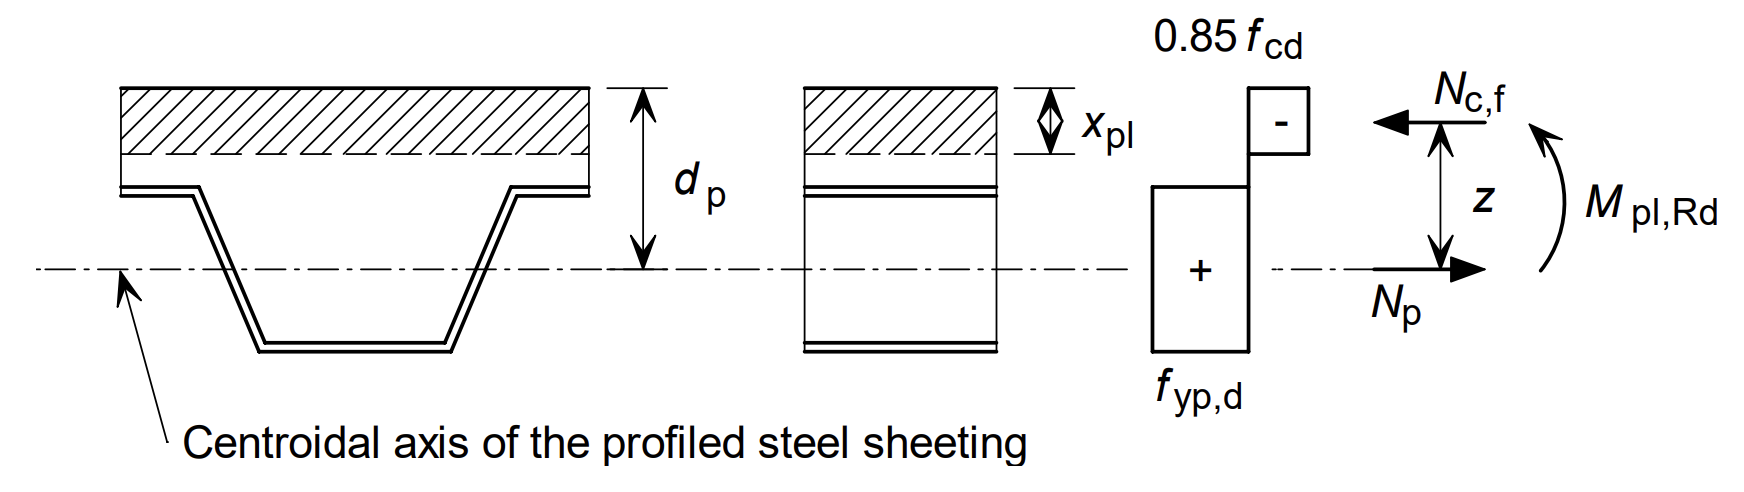
\includegraphics[width=\textwidth]{figures/saggingblockabovesheeting.png}
        \caption{Sagging bending with the plastic neutral axis above the steel sheeting}
        \label{fig:stress_sagging_above}
    \end{subfigure}

    \vspace{1em}

    % --- (b) Sagging, neutral axis within the profile ---
    \begin{subfigure}[t]{0.9\textwidth}
        \centering
        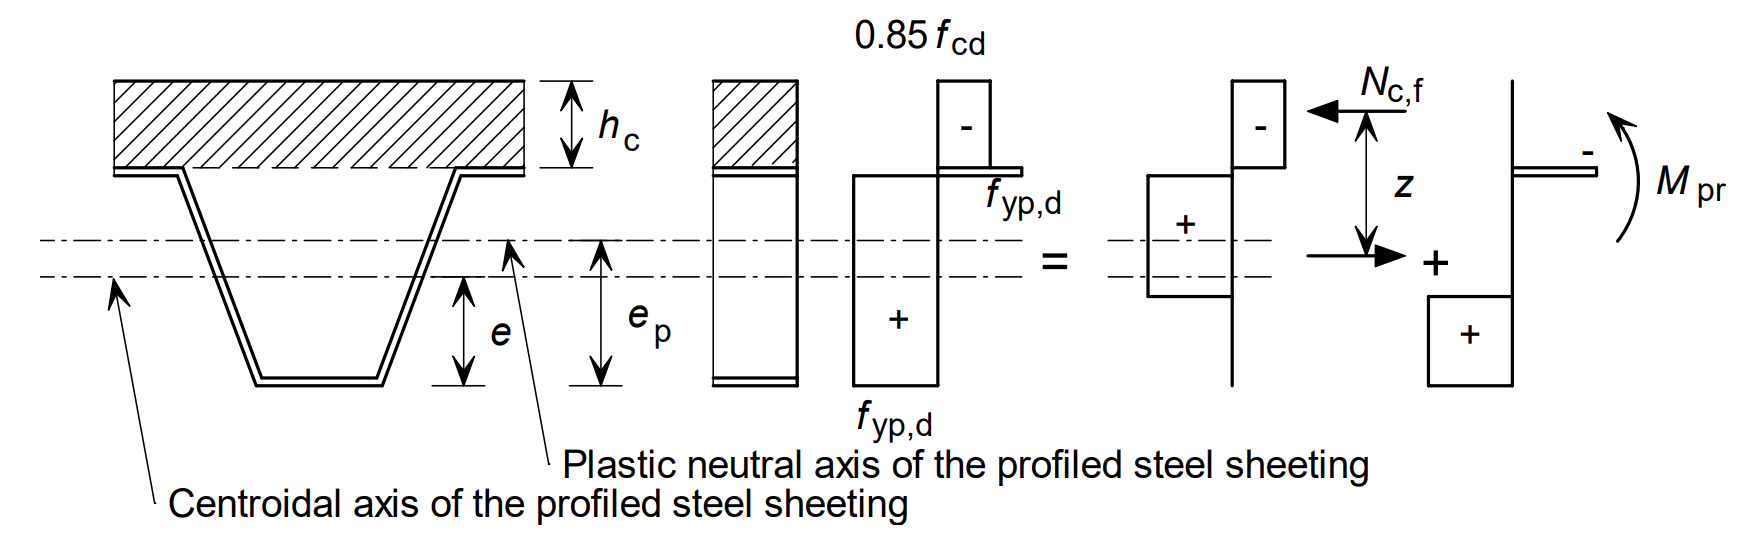
\includegraphics[width=\textwidth]{figures/saggingblockinsheeting.png}
        \caption{Sagging bending with the plastic neutral axis within the steel sheeting}
        \label{fig:stress_sagging_within}
    \end{subfigure}

    \vspace{1em}

    % --- (c) Hogging ---
    \begin{subfigure}[t]{0.9\textwidth}
        \centering
        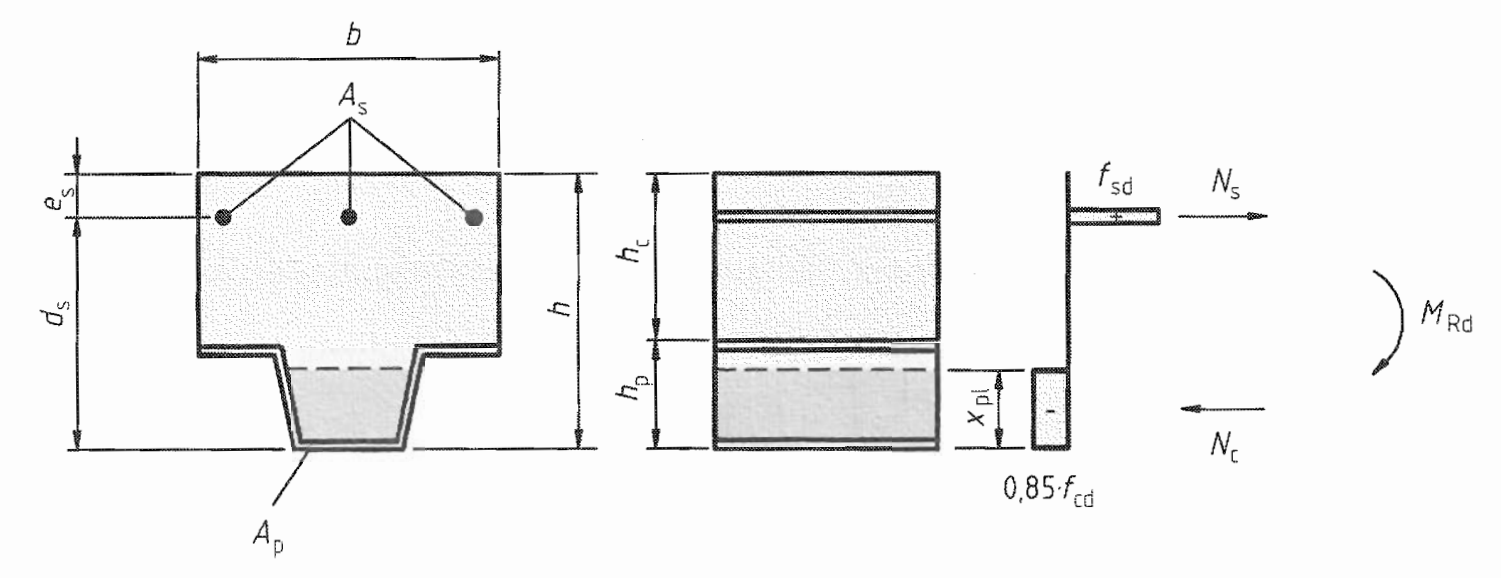
\includegraphics[width=\textwidth]{figures/hoggingblock.png}
        \caption{Hogging bending at an internal support}
        \label{fig:stress_hogging}
    \end{subfigure}

    \caption[Plastic stress distributions for composite slab bending]{Plastic stress distributions used for the ULS moment resistances, reproduced from EN~1994-1-1 Figures~9.5--9.7 \citep{RefWorks:cen2004en4}.}
    \label{fig:stress_blocks}
\end{figure}

\paragraph{Interaction of construction redistribution with composite hogging.}
The decision not to apply plastic redistribution at the construction stage (Section~\ref{sec:constr_stage}) has a consequence for the composite hogging resistance that is worth making explicit. 4-1-1/9.7.3(2)P permits the profiled steel sheeting to be included in the compression zone of the hogging cross-section only where the sheeting is continuous over the support \emph{and} no plastic redistribution of moments has been carried out at the construction stage. Because the present model treats the deck as simply supported during casting and therefore never applies construction-stage redistribution, this condition is always met for continuous configurations: the deck remains eligible to contribute to the composite hogging resistance, as reflected in Equation~\eqref{eq:hogging}. Had construction-stage redistribution been used, the deck would have to be excluded from the hogging calculation, reducing the available hogging resistance and requiring heavier support reinforcement. The simply-supported construction assumption is therefore not merely conservative at the construction stage but also slightly beneficial at the composite stage, since it preserves the deck contribution to hogging.

\paragraph{SLS deflection.}
The composite-stage deflection check uses the transformed composite second moment of area $I_c$, computed about the elastic neutral axis with concrete transformed to steel using the modular ratio $n$:
\begin{equation}
    I_c = \frac{b}{n} \cdot \frac{h_c^3}{12} + \frac{b\,h_c}{n}\left(\bar{y} - h_p - \frac{h_c}{2}\right)^2 + I_{p} + A_{p,e}\,(\bar{y} - e_p)^2
    \label{eq:Ic}
\end{equation}
The short-term modular ratio $n_0 = E_a/E_{cm}$ is used for variable loads; the long-term ratio $n_L = n_0(1 + 1.1\,\varphi_t)$ is used for permanent loads, with the creep coefficient $\varphi_t$ computed from 2-1-1 Annex B using the concrete mean strength $f_{cm} = f_{ck} + 8$\,MPa and the notional size $h_0 = 2\,h_c$. The notional size uses $h_0 = 2 h_c$ rather than $2 A_c / u$ since the steel deck seals the underside of the slab and only the top face is exposed to drying.

The treatment of self-weight deflection differs between propped and unpropped construction:

\begin{itemize}
    \item \textbf{Unpropped.} The deflection from deck self-weight and wet concrete is locked into the construction-stage deflected shape before composite action develops. This locked-in deflection has already been independently verified against $\delta_\mathrm{limit}$ per 4-1-1/9.3.2 (see above). The composite-stage $L/300$ total limit is therefore applied only to \emph{post-composite} deflections --- superimposed-dead load (SDL) and variable loads:
\begin{equation}
    \delta_\mathrm{tot} = \delta_\mathrm{SDL} + \delta_\mathrm{var} \le L/300
    \label{eq:delta_tot_unpropped}
\end{equation}

    \item \textbf{Propped.} Props carry the wet concrete weight during casting; on prop removal the composite section resists the full slab self-weight. The locked-in deflection is therefore zero, and the $L/300$ total limit applies to the sum of self-weight, SDL, and variable deflections --- all computed on the composite section:
\begin{equation}
    \delta_\mathrm{tot} = \delta_\mathrm{SW} + \delta_\mathrm{SDL} + \delta_\mathrm{var} \le L/300
    \label{eq:delta_tot_propped}
\end{equation}
\end{itemize}

In both cases, self-weight and SDL components use the long-term modular ratio $n_L$ to account for creep; the variable-load component uses $n_0$. An independent variable-load limit is also enforced:
\begin{equation}
    \delta_\mathrm{var} \le \min(L/350,\;20\,\mathrm{mm})
\end{equation}

\subsubsection*{Fire design}
\label{sec:fire}

Fire resistance is verified in accordance with 4-1-2 Annex~D, which provides a "model for the calculation of the fire resistance of unprotected composite slabs exposed to fire beneath the slab according to the standard temperature-time curve”. A default fire resistance period of R60 is applied. Four checks are performed in the following order.

\textbf{D1 --- Thermal insulation.} The insulation fire resistance time $t_i$ is calculated from formula D.1 as a function of the concrete depth above the ribs $h_c$, the upper-flange view factor $\Phi$ (formula D.3), the rib geometry factor $A/L_r$ (formula D.2), and the upper-flange width $l_3$, using the coefficient set of Table~D.1 for normal weight concrete:
\begin{equation}
    t_i = a_0 + a_1 h_c + a_2 \Phi + a_3 (A/L_r) + a_4 (1/l_3) + a_5 (A/L_r)(1/l_3)
    \label{eq:fire_d1}
\end{equation}
The check is satisfied when $t_i \ge R_\mathrm{fi}$.

\textbf{D4 --- Minimum effective thickness.} The effective slab thickness $h_\mathrm{eff}$ is computed from formulae D.15a or D.15b depending on the ratio $h_p/h_c$, and compared against the minimum values of Table~D.6. This check is independent of loading.

\textbf{D2 --- Sagging moment resistance.} The fire moment demand $M_\mathrm{Ed,fi}$ is calculated from the accidental load combination of EN~1990, using a fire combination factor $\psi_\mathrm{fi}$ that depends on occupancy. The deck steel temperature at the lower flange, web, and upper flange is calculated from formula D.4 (Table~D.2 coefficients):
\begin{equation}
    \theta_a = b_0 + b_1 (1/l_3) + b_2 (A/L_r) + b_3 \Phi + b_4 \Phi^2
    \label{eq:fire_d4}
\end{equation}
The corresponding strength reduction factor $k_{y,\theta}$ is obtained by linear interpolation through Table~3.2 of EN~1994-1-2. The sagging moment resistance at elevated temperature is then assembled from the deck contribution and the trough bar contribution using a rectangular stress block:
\begin{equation}
    M_\mathrm{Rd,fi} = N_\mathrm{deck,fi} \cdot z_\mathrm{deck} + N_\mathrm{bar,fi} \cdot z_\mathrm{bar}
    \label{eq:mrd_fi}
\end{equation}
where $N_\mathrm{deck,fi} = A_{p,e} \cdot f_{ypd} \cdot k_{y,\theta,\mathrm{deck}}$ and $N_\mathrm{bar,fi} = A_{s,\mathrm{tr}} \cdot f_{sk} \cdot k_{y,\theta,\mathrm{bar}}$.

Trough bar selection is carried out iteratively. Bar diameters of 8, 10, 12, 16, and 20\,mm are evaluated in ascending order. Each bar is assumed to be located at the geometric centre of the trough cross-section, with axis distances $u_1$ and $u_2$ derived from this central position; the axis distance $u_3$ from the lower flange is taken as 25\,mm for shallow profiles or 70\,mm for deep profiles. The temperature of each candidate bar is determined from formula D.5:
\begin{equation}
    \theta_s = c_0 + c_1 (u_3/h_p) + c_2 \sqrt{z} + c_3 (A/L_r) + c_4 \alpha + c_5 (1/l_3)
    \label{eq:fire_d5}
\end{equation}
where the position factor $z = 1/(1/\sqrt{u_1} + 1/\sqrt{u_2} + 1/\sqrt{u_3})$ and $\alpha$ is the web inclination. The smallest diameter for which $M_\mathrm{Rd,fi} \ge M_\mathrm{Ed,fi}$ is selected; if no diameter satisfies the check, the cross-section is recorded as failing D2.

\textbf{D3 --- Hogging moment at internal supports.} For continuous configurations only ($n_\mathrm{spans} > 1$), the reduced concrete compression zone depth due to isotherm penetration $b$ is determined by a single forward pass following the procedure of Annex~D.3: the limiting mesh temperature $\theta_\mathrm{lim}$ is obtained from formula D.7 (Table~D.4 coefficients), the position factor $z$ is inverted from formula D.5 using $u_3/h_p = 0.75$ (the value explicitly permitted by Annex~D.3 Note~6), and the isotherm penetration depth into the solid zone above the ribs is derived from formula D.11. The check is satisfied when the reduced-section hogging moment resistance $M_\mathrm{Rd,fi}$ equals or exceeds the fire hogging demand. The top mesh reinforcement on the unexposed face is assumed to remain at ambient temperature.

\subsubsection*{Vibration}
\label{sec:vibration_method}

Vibration serviceability is not incorporated as a structural constraint within the main optimisation. The Steel Construction Institute (SCI) publication 354 \citep{RefWorks:hicks2009p354} outlines the design guidance for all types of floor construction involving steel for determining the vibration response of sensitive floors. It is widely used in practice and allows the floor response to be compared with other UK documents such as BS 6472 and ISO 10137. The document was carried out as part of the ECSC project involving RWTH and Arcelor Profil Luxembourg Research.

The full method outlined in section 7 of this publication requires bay-level geometry inputs --- secondary beam span, primary beam span, bay width, and damping ratio --- none of which are defined in a slab-only optimisation study. Including a beam model would introduce multiple additional discrete variables (beam section, bay geometry) and fundamentally change the scope of the comparison, which is limited to the slab cross-section.
 
Instead, a slab-only screening check is performed as a post-processing step (implemented in \texttt{verify\_vibration.py}). The slab is modelled as a 1\,m-wide, simply-supported strip spanning the secondary-beam spacing $b$ on rigid supports, isolating the slab's own contribution to the floor frequency; this is the quantity reported by the ComFlor design tool, and it follows the SCI~P354 approach. The check proceeds in three steps.
 
First, the dynamic second moment of area of the slab strip is obtained from the power-law fit to SCI~P354 Table~7.2 for normal-weight concrete:
\begin{equation}
    I_s = c\, h_s^{3.7} \quad [\mathrm{mm^4/m}]
    \label{eq:vib_Is}
\end{equation}
where $h_s$ is the slab depth and $c$ is the Table~7.2 coefficient interpolated by rib height $h_p$ ($c = 0.37$ for re-entrant profiles; $c = 0.23$, $0.19$, and $0.05$ for trapezoidal profiles at $h_p \le 60$, $80$, and $225$\,mm respectively, linearly interpolated).
 
Second, the mid-span deflection of the simply-supported strip under the vibrating mass is computed:
\begin{equation}
    \delta = \frac{5\, m\, g\, b^4}{384\, EI_s} \quad [\mathrm{m}]
    \label{eq:vib_delta}
\end{equation}
where the floor mass per unit area is taken as the permanent load plus 10\% of the imposed load, with partitions excluded, in accordance with SCI~P354 4.1.2:
\begin{equation}
    m = \left(SW + \mathrm{SDL} + 0.1\, Q_k\right) \cdot 1000 / g \quad [\mathrm{kg/m^2}]
    \label{eq:vib_mass}
\end{equation}
The slab self-weight is computed consistently with the main optimiser from the profiled (average) concrete depth plus the deck sheeting. The superimposed and imposed loads match the office scenario, with $\mathrm{SDL} = 1.105$\,kN/m\textsuperscript{2} ($0.355$\,kN/m\textsuperscript{2} finishes $+\ 0.75$\,kN/m\textsuperscript{2} services) and $Q_k = 2.5$\,kN/m\textsuperscript{2}.
 
Third, the fundamental frequency is obtained from the resulting deflection using SCI~P354 Eq.~4:
\begin{equation}
    f_1 = \frac{18}{\sqrt{\delta_\mathrm{mm}}} \quad [\mathrm{Hz}]
    \label{eq:vib_f1}
\end{equation}
where $\delta_\mathrm{mm}$ is the mid-span deflection of Equation~\eqref{eq:vib_delta} expressed in millimetres. The slab is assessed against $f_1 \ge 3$\,Hz, the absolute SCI~P354 minimum for floor elements to avoid resonance due to walking.
 
This slab-only frequency is deliberately conservative as a screening check: the frequency of the complete floor, in which the slab is supported on flexible beams rather than rigid supports, is always \emph{lower} than the slab-alone value, because the beam flexibility adds to the total deflection. Passing the slab-only check is therefore necessary but not sufficient --- a floor that passes here may still fail once beam flexibility is included. The full system response-factor check, which accounts for beam and bay participation, modal mass, and damping, is implemented separately in \texttt{full\_vibration\_check.py}; a representative worked example of that full check is given in Appendix~\ref{app:vibration} to illustrate the procedure and to show the extent to which the full-floor frequency falls below the slab-alone screening value.
 
At longer office spans, vibration is likely to govern the overall composite floor design once beams are also considered. The implications are discussed further in Section~\ref{sec:assumptions}.

\todo[inline]{Add full bay configuration example to appendix.}

\subsubsection*{Acoustic performance}
\label{sec:acoustic}

Acoustic performance is not incorporated as a structural constraint within the optimisation. Instead, the floor build-up for each occupancy scenario (Table~\ref{tab:floor_buildup}) is pre-selected to meet the applicable acoustic requirements, and its GWP contribution is added to $\mathrm{GWP}_\mathrm{total}$ as described in Section~\ref{sec:env_impact}.

The two phenomena of concern are airborne sound transmission and impact sound transmission. In Switzerland, SIA~181 \citep{RefWorks:sia181} expresses its requirements using a standardised level difference $D_i$ for airborne sound and a standardised impact sound pressure level $L'_i$ for impact sound, set according to a classification of the sensitivity of the receiving space and the noise exposure.  In the United Kingdom, Approved Document~E \citep{RefWorks:adePartE} specifies field-measured requirements for separating floors for the standardised weighted sound level difference including a spectrum adaptation term ($D_{nT,w}+C_\mathrm{tr}$) and standrdised weighted impact sound preseure ($L'_{nT,w}$) levels. The requirements for each use case are given in Table~.

\todo[inline]{Add table of the requirements from word document 'acoustic checks'}

\todo[inline]{Explain method for making the floor build ups.}

The acoustic performance of each floor build up was estimated using the SCI publications 321 \citep{RefWorks:RefID:acousticslimdek} and 322 \citep{RefWorks:acousticcomposite}.

For the \textbf{office} scenario, the build-up consists of a raised access floor system comprising a chipboard panel (18\,mm), gypsum fibreboard (19\,mm), and rock wool insulation (30\,mm). Raised access floors are widely used in commercial office fit-out to route mechanical and electrical services and are compatible with composite slab construction without structural modifications.

For the \textbf{residential} scenario, the build-up comprises a two-layer factory-sealed parquet (11\,mm) over a cement screed (85\,mm) and glass wool insulation (30\,mm). For the \textbf{retail} scenario, a parquet finish over gypsum fibreboard and glass wool insulation is adopted. For the \textbf{industrial} scenario, a cement screed over rock wool insulation provides impact damping with minimal additional GWP. 

%===============================================================
\subsection{Environmental impact}
\label{sec:env_impact}
%===============================================================
The environmental impact of each cross-section is quantified as Global Warming Potential per metre of span length (kg\,CO$_2$-eq/m). The assessment covers EN~15804 modules A1--A3 (raw material supply, transport to factory, manufacturing) and modules C1--C4 (deconstruction, transport, waste processing, disposal). Modules A4--A5, B1--B7, and D are excluded as they introduce project-specific assumptions incompatible with early-stage comparative assessment.

The structural GWP is computed as the sum of four material contributions:
\begin{equation}
    \mathrm{GWP}_\mathrm{structure} = \rho_c \, h_\mathrm{c,avg} \, \mathrm{GWP}_c + \mathrm{GWP}_\mathrm{deck} + A_s \, \rho_s \, \mathrm{GWP}_s + A_{s,\mathrm{tr}} \, \rho_s \, \mathrm{GWP}_s
    \label{eq:gwp_structure}
\end{equation}

where $\rho_c$ and $\rho_s$ are the dry densities of concrete and reinforcing steel respectively; $A_s$ is the mesh cross-sectional area per unit width; $A_{s,\mathrm{tr}}$ is the trough bar area per unit width introduced by the fire check (zero if no trough bars are required); and $\mathrm{GWP}_c$, $\mathrm{GWP}_s$, and $\mathrm{GWP}_\mathrm{deck}$ are the GWP values drawn from the product database. The average concrete depth $h_\mathrm{c,avg}$ accounts for both the concrete above the ribs and the concrete that fills the trough voids:
\begin{equation}
    h_\mathrm{c,avg} = h_c + V_\mathrm{tr}
    \label{eq:hcavg}
\end{equation}
where $V_\mathrm{tr}$ is the trough concrete volume per unit plan area (m$^3$/m$^2$), sourced from the manufacturer database.

The deck contribution $\mathrm{GWP}_\mathrm{deck}$ is normalised to a per-metre-length basis before summation. Where the manufacturer EPD is expressed per unit area, the value is multiplied by the unit strip width of 1\,m. Where the EPD is expressed per unit mass, the value is converted using the manufacturer-declared deck weight per unit area:
\begin{equation}
    \mathrm{GWP}_\mathrm{deck} = 
    \begin{cases}
    \mathrm{GWP}_\mathrm{deck}^{(\mathrm{m}^2)} \cdot b           & \text{if EPD per m}^2 \\
    w_\mathrm{deck} \cdot \mathrm{GWP}_\mathrm{deck}^{(\mathrm{kg})} \cdot b & \text{if EPD per kg or per t}
    \end{cases}
    \label{eq:gwp_deck_norm}
\end{equation}
where $w_\mathrm{deck}$ is the deck weight in kg/m$^2$ and $b = 1$\,m is the strip width.

The total GWP is obtained by adding the contribution of the non-structural floor build-up to the structural cross-section:
\begin{equation}
    \mathrm{GWP}_\mathrm{total} = \mathrm{GWP}_\mathrm{structure} + \sum_{i \in \mathrm{layers}} \rho_i \, t_i \, \mathrm{GWP}_i
    \label{eq:gwp_total}
\end{equation}
where the sum runs over all layers in the floor build-up table for the relevant occupancy scenario (Table~\ref{tab:floor_buildup}), and $\rho_i$, $t_i$, $\mathrm{GWP}_i$ are the layer density, thickness, and GWP value respectively.

%===============================================================
\subsection{Optimisation}
\label{sec:optimisation}
%===============================================================
The optimisation of composite slab cross-sections differs from the approach used for the reinforced concrete and timber baselines in the pre-existing framework. Because the composite slab has a single continuous design variable --- the total slab depth $h$ --- a scalar bounded optimisation is both sufficient and substantially more efficient than the multi-variable basin-hopping approach used for the RC and timber classes. The complete workflow is shown in Figure~\ref{fig:code_flowchart}, in which the boxes are coloured by the source module responsible for each stage.

\begin{figure}[p]
  \centering
  \resizebox{\textwidth}{!}{% ============================================================================
%  Composite slab optimisation workflow — flowchart for the Methodology chapter
%  Boxes are colour-coded by source module; each box is tagged with the
%  script and the class / function used at that stage.
%
%  Requires in MAIN.tex preamble:
%     \usepackage{tikz}
%     \usetikzlibrary{shapes.geometric, arrows.meta, positioning, calc, fit, backgrounds}
%  Then include with:  % ============================================================================
%  Composite slab optimisation workflow — flowchart for the Methodology chapter
%  Boxes are colour-coded by source module; each box is tagged with the
%  script and the class / function used at that stage.
%
%  Requires in MAIN.tex preamble:
%     \usepackage{tikz}
%     \usetikzlibrary{shapes.geometric, arrows.meta, positioning, calc, fit, backgrounds}
%  Then include with:  % ============================================================================
%  Composite slab optimisation workflow — flowchart for the Methodology chapter
%  Boxes are colour-coded by source module; each box is tagged with the
%  script and the class / function used at that stage.
%
%  Requires in MAIN.tex preamble:
%     \usepackage{tikz}
%     \usetikzlibrary{shapes.geometric, arrows.meta, positioning, calc, fit, backgrounds}
%  Then include with:  \input{code_flowchart}   (inside a figure environment)
% ============================================================================
\begin{tikzpicture}[
    font=\footnotesize,
    node distance = 4mm and 10mm,
    >={Stealth[length=2.2mm]},
    line/.style   = {draw, ->, thick, rounded corners},
    % --- module colours ---
    entry/.style  = {rectangle, rounded corners=4pt, draw=violet!70, fill=violet!8,
                     text width=44mm, align=center, inner sep=3pt},
    driver/.style = {rectangle, draw=orange!85!black, fill=orange!12,
                     text width=48mm, align=center, inner sep=3pt},
    optim/.style  = {rectangle, draw=green!55!black, fill=green!10,
                     text width=52mm, align=center, inner sep=3pt},
    analysis/.style = {rectangle, draw=blue!70, fill=blue!8,
                     text width=52mm, align=center, inner sep=3pt},
    startstop/.style = {rectangle, rounded corners=7pt, draw=black!70, fill=black!8,
                     text width=30mm, align=center, inner sep=3pt},
    decision/.style = {diamond, aspect=2.2, draw=red!60!black, fill=red!7,
                     text width=24mm, align=center, inner sep=1pt},
    check/.style  = {rectangle, draw=blue!55, fill=blue!4, text width=64mm,
                     align=left, inner sep=4pt, font=\scriptsize},
]

% ---- main vertical spine -------------------------------------------------
\node[startstop] (start) {\textbf{Start}};

\node[entry, below=of start] (inputs)
   {Define inputs: occupancy, loads,\\ fire rating $R_\mathrm{fi}$, $\psi_\mathrm{fi}$, build-up\\
    {\ttfamily\scriptsize simple/two/three\_span\_composite.py}\\ {\ttfamily\scriptsize FloorStruc}};

\node[driver, below=of inputs] (cfg)
   {\textbf{For each} span configuration (1, 2, 3 spans)\\
    {\ttfamily\scriptsize run\_dataset() · n\_spans}};

\node[driver, below=of cfg] (span)
   {\textbf{For each} span $L$ (3--10\,m)\\
    {\ttfamily\scriptsize plot\_datasets.py · \_build\_member\_list()}};

\node[driver, below=of span] (deck)
   {\textbf{For each} deck product \& concrete grade\\ {\scriptsize(Tata Steel, Kingspan; C25/30, C30/37)}\\
    {\ttfamily\scriptsize Decking · ReadyMixedConcrete}};

\node[optim, below=of deck] (opt)
   {\textbf{Optimise depth $h$}\\ \texttt{minimize\_scalar} (Brent), minimise GWP\\ {\scriptsize(penalty for constraint violations)}\\
    {\ttfamily\scriptsize struct\_optimization.py}\\ {\ttfamily\scriptsize opt\_comp\_slab() · comp\_slab\_rqs()}};

\node[analysis, below=of opt] (checks)
   {\textbf{Evaluate all limit states}\\
    {\ttfamily\scriptsize struct\_analysis.py}\\ {\ttfamily\scriptsize CompositeSlab.run\_all\_checks()}};

\node[decision, below=of checks] (feas) {All checks pass?};

\node[driver, below=5mm of feas] (record)
   {Record GWP, $h$, deck, propped status, governing check\\
    {\ttfamily\scriptsize \_CompSlabMember}};

\node[decision, below=of record]   (moredeck) {More deck/\\ concrete?};
\node[decision, below=of moredeck]  (morespan) {More spans?};
\node[decision, below=of morespan]  (morecfg)  {More configs?};

\node[driver, below=of morecfg] (out)
   {\textbf{Outputs:} min-GWP section per span;\\ GWP-vs-span plots vs RC/timber;\\ governing-check \& breakdown data\\
    {\ttfamily\scriptsize plot\_from\_csv() · \_save\_to\_csv()}};

\node[startstop, below=of out] (stop) {\textbf{End}};

% ---- spine arrows --------------------------------------------------------
\draw[line] (start) -- (inputs);
\draw[line] (inputs) -- (cfg);
\draw[line] (cfg) -- (span);
\draw[line] (span) -- (deck);
\draw[line] (deck) -- (opt);
\draw[line] (opt) -- (checks);
\draw[line] (checks) -- (feas);
\draw[line] (feas) -- node[right, font=\scriptsize] {yes} (record);
\draw[line] (record) -- (moredeck);
\draw[line] (moredeck) -- node[right, font=\scriptsize] {no} (morespan);
\draw[line] (morespan) -- node[right, font=\scriptsize] {no} (morecfg);
\draw[line] (morecfg) -- node[right, font=\scriptsize] {no} (out);
\draw[line] (out) -- (stop);

% ---- feasibility "no" -> propped retry -----------------------------------
\node[optim, right=12mm of feas, text width=34mm] (propped)
   {Retry with \textbf{propped} construction {\scriptsize(if unpropped infeasible)}\\
    {\ttfamily\scriptsize opt\_comp\_slab(propped=True)}};
\draw[line] (feas.east) -- node[above, font=\scriptsize] {no} (propped.west);
\draw[line] (propped.north) |- ($(checks.east)+(0,2mm)$);

% ---- loop-back arrows ----------------------------------------------------
\draw[line] (moredeck.west) -- node[above, font=\scriptsize] {yes} ++(-24mm,0) |- (deck.west);
\draw[line] (morespan.west) -- node[above, font=\scriptsize] {yes} ++(-36mm,0) |- (span.west);
\draw[line] (morecfg.west)  -- node[below, font=\scriptsize, pos=0.25] {yes} ++(-48mm,0) |- (cfg.west);

% ---- run_all_checks expansion (right callout) ----------------------------
\node[check, right=44mm of opt, anchor=north west] (cklist)
  {\textbf{\texttt{CompositeSlab.run\_all\_checks()}} \hfill {\scriptsize\itshape struct\_analysis.py}\\
   {\scriptsize via the \texttt{\_chk\_*} methods:}\\[2pt]
   \textit{Construction stage (unpropped only)}\\
   \;$\bullet$ ULS deck bending \;\; $\bullet$ ULS web shear\\
   \;$\bullet$ SLS deflection (+ ponding)\\[2pt]
   \textit{Composite stage}\\
   \;$\bullet$ ULS sagging moment\\
   \;$\bullet$ ULS longitudinal shear (m--k / $\tau_u$)\\
   \;$\bullet$ ULS vertical shear\\
   \;$\bullet$ ULS hogging (continuous spans)\\
   \;$\bullet$ SLS deflection ($L/300$)\\[2pt]
   \textit{Fire — EN 1994-1-2 Annex D (if $R_\mathrm{fi}\!>\!0$)}\\
   \;$\bullet$ D1 insulation\\
   \;$\bullet$ D2 sagging (+ trough bar selection)\\
   \;$\bullet$ D3 hogging (continuous spans)\\
   \;$\bullet$ D4 min.\ effective thickness\\
   \;$\bullet$ D5 field of application};
\draw[densely dashed, gray] (checks.east) -- (cklist.west);

% ---- module legend (bottom-right) ----------------------------------------
\node[check, draw=black!45, fill=white, text width=58mm, below=8mm of cklist.south west, anchor=north west] (legend)
  {\textbf{Module key (colour)}\\[2pt]
   \tikz\fill[violet!8,draw=violet!70](0,0)rectangle(2.6mm,2.6mm); \; \texttt{*\_span\_composite.py} — entry / setup\\
   \tikz\fill[orange!12,draw=orange!85!black](0,0)rectangle(2.6mm,2.6mm); \; \texttt{plot\_datasets.py} — driver: loops, I/O\\
   \tikz\fill[green!10,draw=green!55!black](0,0)rectangle(2.6mm,2.6mm); \; \texttt{struct\_optimization.py} — optimiser\\
   \tikz\fill[blue!8,draw=blue!70](0,0)rectangle(2.6mm,2.6mm); \; \texttt{struct\_analysis.py} — cross-section \& checks};

\end{tikzpicture}
   (inside a figure environment)
% ============================================================================
\begin{tikzpicture}[
    font=\footnotesize,
    node distance = 4mm and 10mm,
    >={Stealth[length=2.2mm]},
    line/.style   = {draw, ->, thick, rounded corners},
    % --- module colours ---
    entry/.style  = {rectangle, rounded corners=4pt, draw=violet!70, fill=violet!8,
                     text width=44mm, align=center, inner sep=3pt},
    driver/.style = {rectangle, draw=orange!85!black, fill=orange!12,
                     text width=48mm, align=center, inner sep=3pt},
    optim/.style  = {rectangle, draw=green!55!black, fill=green!10,
                     text width=52mm, align=center, inner sep=3pt},
    analysis/.style = {rectangle, draw=blue!70, fill=blue!8,
                     text width=52mm, align=center, inner sep=3pt},
    startstop/.style = {rectangle, rounded corners=7pt, draw=black!70, fill=black!8,
                     text width=30mm, align=center, inner sep=3pt},
    decision/.style = {diamond, aspect=2.2, draw=red!60!black, fill=red!7,
                     text width=24mm, align=center, inner sep=1pt},
    check/.style  = {rectangle, draw=blue!55, fill=blue!4, text width=64mm,
                     align=left, inner sep=4pt, font=\scriptsize},
]

% ---- main vertical spine -------------------------------------------------
\node[startstop] (start) {\textbf{Start}};

\node[entry, below=of start] (inputs)
   {Define inputs: occupancy, loads,\\ fire rating $R_\mathrm{fi}$, $\psi_\mathrm{fi}$, build-up\\
    {\ttfamily\scriptsize simple/two/three\_span\_composite.py}\\ {\ttfamily\scriptsize FloorStruc}};

\node[driver, below=of inputs] (cfg)
   {\textbf{For each} span configuration (1, 2, 3 spans)\\
    {\ttfamily\scriptsize run\_dataset() · n\_spans}};

\node[driver, below=of cfg] (span)
   {\textbf{For each} span $L$ (3--10\,m)\\
    {\ttfamily\scriptsize plot\_datasets.py · \_build\_member\_list()}};

\node[driver, below=of span] (deck)
   {\textbf{For each} deck product \& concrete grade\\ {\scriptsize(Tata Steel, Kingspan; C25/30, C30/37)}\\
    {\ttfamily\scriptsize Decking · ReadyMixedConcrete}};

\node[optim, below=of deck] (opt)
   {\textbf{Optimise depth $h$}\\ \texttt{minimize\_scalar} (Brent), minimise GWP\\ {\scriptsize(penalty for constraint violations)}\\
    {\ttfamily\scriptsize struct\_optimization.py}\\ {\ttfamily\scriptsize opt\_comp\_slab() · comp\_slab\_rqs()}};

\node[analysis, below=of opt] (checks)
   {\textbf{Evaluate all limit states}\\
    {\ttfamily\scriptsize struct\_analysis.py}\\ {\ttfamily\scriptsize CompositeSlab.run\_all\_checks()}};

\node[decision, below=of checks] (feas) {All checks pass?};

\node[driver, below=5mm of feas] (record)
   {Record GWP, $h$, deck, propped status, governing check\\
    {\ttfamily\scriptsize \_CompSlabMember}};

\node[decision, below=of record]   (moredeck) {More deck/\\ concrete?};
\node[decision, below=of moredeck]  (morespan) {More spans?};
\node[decision, below=of morespan]  (morecfg)  {More configs?};

\node[driver, below=of morecfg] (out)
   {\textbf{Outputs:} min-GWP section per span;\\ GWP-vs-span plots vs RC/timber;\\ governing-check \& breakdown data\\
    {\ttfamily\scriptsize plot\_from\_csv() · \_save\_to\_csv()}};

\node[startstop, below=of out] (stop) {\textbf{End}};

% ---- spine arrows --------------------------------------------------------
\draw[line] (start) -- (inputs);
\draw[line] (inputs) -- (cfg);
\draw[line] (cfg) -- (span);
\draw[line] (span) -- (deck);
\draw[line] (deck) -- (opt);
\draw[line] (opt) -- (checks);
\draw[line] (checks) -- (feas);
\draw[line] (feas) -- node[right, font=\scriptsize] {yes} (record);
\draw[line] (record) -- (moredeck);
\draw[line] (moredeck) -- node[right, font=\scriptsize] {no} (morespan);
\draw[line] (morespan) -- node[right, font=\scriptsize] {no} (morecfg);
\draw[line] (morecfg) -- node[right, font=\scriptsize] {no} (out);
\draw[line] (out) -- (stop);

% ---- feasibility "no" -> propped retry -----------------------------------
\node[optim, right=12mm of feas, text width=34mm] (propped)
   {Retry with \textbf{propped} construction {\scriptsize(if unpropped infeasible)}\\
    {\ttfamily\scriptsize opt\_comp\_slab(propped=True)}};
\draw[line] (feas.east) -- node[above, font=\scriptsize] {no} (propped.west);
\draw[line] (propped.north) |- ($(checks.east)+(0,2mm)$);

% ---- loop-back arrows ----------------------------------------------------
\draw[line] (moredeck.west) -- node[above, font=\scriptsize] {yes} ++(-24mm,0) |- (deck.west);
\draw[line] (morespan.west) -- node[above, font=\scriptsize] {yes} ++(-36mm,0) |- (span.west);
\draw[line] (morecfg.west)  -- node[below, font=\scriptsize, pos=0.25] {yes} ++(-48mm,0) |- (cfg.west);

% ---- run_all_checks expansion (right callout) ----------------------------
\node[check, right=44mm of opt, anchor=north west] (cklist)
  {\textbf{\texttt{CompositeSlab.run\_all\_checks()}} \hfill {\scriptsize\itshape struct\_analysis.py}\\
   {\scriptsize via the \texttt{\_chk\_*} methods:}\\[2pt]
   \textit{Construction stage (unpropped only)}\\
   \;$\bullet$ ULS deck bending \;\; $\bullet$ ULS web shear\\
   \;$\bullet$ SLS deflection (+ ponding)\\[2pt]
   \textit{Composite stage}\\
   \;$\bullet$ ULS sagging moment\\
   \;$\bullet$ ULS longitudinal shear (m--k / $\tau_u$)\\
   \;$\bullet$ ULS vertical shear\\
   \;$\bullet$ ULS hogging (continuous spans)\\
   \;$\bullet$ SLS deflection ($L/300$)\\[2pt]
   \textit{Fire — EN 1994-1-2 Annex D (if $R_\mathrm{fi}\!>\!0$)}\\
   \;$\bullet$ D1 insulation\\
   \;$\bullet$ D2 sagging (+ trough bar selection)\\
   \;$\bullet$ D3 hogging (continuous spans)\\
   \;$\bullet$ D4 min.\ effective thickness\\
   \;$\bullet$ D5 field of application};
\draw[densely dashed, gray] (checks.east) -- (cklist.west);

% ---- module legend (bottom-right) ----------------------------------------
\node[check, draw=black!45, fill=white, text width=58mm, below=8mm of cklist.south west, anchor=north west] (legend)
  {\textbf{Module key (colour)}\\[2pt]
   \tikz\fill[violet!8,draw=violet!70](0,0)rectangle(2.6mm,2.6mm); \; \texttt{*\_span\_composite.py} — entry / setup\\
   \tikz\fill[orange!12,draw=orange!85!black](0,0)rectangle(2.6mm,2.6mm); \; \texttt{plot\_datasets.py} — driver: loops, I/O\\
   \tikz\fill[green!10,draw=green!55!black](0,0)rectangle(2.6mm,2.6mm); \; \texttt{struct\_optimization.py} — optimiser\\
   \tikz\fill[blue!8,draw=blue!70](0,0)rectangle(2.6mm,2.6mm); \; \texttt{struct\_analysis.py} — cross-section \& checks};

\end{tikzpicture}
   (inside a figure environment)
% ============================================================================
\begin{tikzpicture}[
    font=\footnotesize,
    node distance = 4mm and 10mm,
    >={Stealth[length=2.2mm]},
    line/.style   = {draw, ->, thick, rounded corners},
    % --- module colours ---
    entry/.style  = {rectangle, rounded corners=4pt, draw=violet!70, fill=violet!8,
                     text width=44mm, align=center, inner sep=3pt},
    driver/.style = {rectangle, draw=orange!85!black, fill=orange!12,
                     text width=48mm, align=center, inner sep=3pt},
    optim/.style  = {rectangle, draw=green!55!black, fill=green!10,
                     text width=52mm, align=center, inner sep=3pt},
    analysis/.style = {rectangle, draw=blue!70, fill=blue!8,
                     text width=52mm, align=center, inner sep=3pt},
    startstop/.style = {rectangle, rounded corners=7pt, draw=black!70, fill=black!8,
                     text width=30mm, align=center, inner sep=3pt},
    decision/.style = {diamond, aspect=2.2, draw=red!60!black, fill=red!7,
                     text width=24mm, align=center, inner sep=1pt},
    check/.style  = {rectangle, draw=blue!55, fill=blue!4, text width=64mm,
                     align=left, inner sep=4pt, font=\scriptsize},
]

% ---- main vertical spine -------------------------------------------------
\node[startstop] (start) {\textbf{Start}};

\node[entry, below=of start] (inputs)
   {Define inputs: occupancy, loads,\\ fire rating $R_\mathrm{fi}$, $\psi_\mathrm{fi}$, build-up\\
    {\ttfamily\scriptsize simple/two/three\_span\_composite.py}\\ {\ttfamily\scriptsize FloorStruc}};

\node[driver, below=of inputs] (cfg)
   {\textbf{For each} span configuration (1, 2, 3 spans)\\
    {\ttfamily\scriptsize run\_dataset() · n\_spans}};

\node[driver, below=of cfg] (span)
   {\textbf{For each} span $L$ (3--10\,m)\\
    {\ttfamily\scriptsize plot\_datasets.py · \_build\_member\_list()}};

\node[driver, below=of span] (deck)
   {\textbf{For each} deck product \& concrete grade\\ {\scriptsize(Tata Steel, Kingspan; C25/30, C30/37)}\\
    {\ttfamily\scriptsize Decking · ReadyMixedConcrete}};

\node[optim, below=of deck] (opt)
   {\textbf{Optimise depth $h$}\\ \texttt{minimize\_scalar} (Brent), minimise GWP\\ {\scriptsize(penalty for constraint violations)}\\
    {\ttfamily\scriptsize struct\_optimization.py}\\ {\ttfamily\scriptsize opt\_comp\_slab() · comp\_slab\_rqs()}};

\node[analysis, below=of opt] (checks)
   {\textbf{Evaluate all limit states}\\
    {\ttfamily\scriptsize struct\_analysis.py}\\ {\ttfamily\scriptsize CompositeSlab.run\_all\_checks()}};

\node[decision, below=of checks] (feas) {All checks pass?};

\node[driver, below=5mm of feas] (record)
   {Record GWP, $h$, deck, propped status, governing check\\
    {\ttfamily\scriptsize \_CompSlabMember}};

\node[decision, below=of record]   (moredeck) {More deck/\\ concrete?};
\node[decision, below=of moredeck]  (morespan) {More spans?};
\node[decision, below=of morespan]  (morecfg)  {More configs?};

\node[driver, below=of morecfg] (out)
   {\textbf{Outputs:} min-GWP section per span;\\ GWP-vs-span plots vs RC/timber;\\ governing-check \& breakdown data\\
    {\ttfamily\scriptsize plot\_from\_csv() · \_save\_to\_csv()}};

\node[startstop, below=of out] (stop) {\textbf{End}};

% ---- spine arrows --------------------------------------------------------
\draw[line] (start) -- (inputs);
\draw[line] (inputs) -- (cfg);
\draw[line] (cfg) -- (span);
\draw[line] (span) -- (deck);
\draw[line] (deck) -- (opt);
\draw[line] (opt) -- (checks);
\draw[line] (checks) -- (feas);
\draw[line] (feas) -- node[right, font=\scriptsize] {yes} (record);
\draw[line] (record) -- (moredeck);
\draw[line] (moredeck) -- node[right, font=\scriptsize] {no} (morespan);
\draw[line] (morespan) -- node[right, font=\scriptsize] {no} (morecfg);
\draw[line] (morecfg) -- node[right, font=\scriptsize] {no} (out);
\draw[line] (out) -- (stop);

% ---- feasibility "no" -> propped retry -----------------------------------
\node[optim, right=12mm of feas, text width=34mm] (propped)
   {Retry with \textbf{propped} construction {\scriptsize(if unpropped infeasible)}\\
    {\ttfamily\scriptsize opt\_comp\_slab(propped=True)}};
\draw[line] (feas.east) -- node[above, font=\scriptsize] {no} (propped.west);
\draw[line] (propped.north) |- ($(checks.east)+(0,2mm)$);

% ---- loop-back arrows ----------------------------------------------------
\draw[line] (moredeck.west) -- node[above, font=\scriptsize] {yes} ++(-24mm,0) |- (deck.west);
\draw[line] (morespan.west) -- node[above, font=\scriptsize] {yes} ++(-36mm,0) |- (span.west);
\draw[line] (morecfg.west)  -- node[below, font=\scriptsize, pos=0.25] {yes} ++(-48mm,0) |- (cfg.west);

% ---- run_all_checks expansion (right callout) ----------------------------
\node[check, right=44mm of opt, anchor=north west] (cklist)
  {\textbf{\texttt{CompositeSlab.run\_all\_checks()}} \hfill {\scriptsize\itshape struct\_analysis.py}\\
   {\scriptsize via the \texttt{\_chk\_*} methods:}\\[2pt]
   \textit{Construction stage (unpropped only)}\\
   \;$\bullet$ ULS deck bending \;\; $\bullet$ ULS web shear\\
   \;$\bullet$ SLS deflection (+ ponding)\\[2pt]
   \textit{Composite stage}\\
   \;$\bullet$ ULS sagging moment\\
   \;$\bullet$ ULS longitudinal shear (m--k / $\tau_u$)\\
   \;$\bullet$ ULS vertical shear\\
   \;$\bullet$ ULS hogging (continuous spans)\\
   \;$\bullet$ SLS deflection ($L/300$)\\[2pt]
   \textit{Fire — EN 1994-1-2 Annex D (if $R_\mathrm{fi}\!>\!0$)}\\
   \;$\bullet$ D1 insulation\\
   \;$\bullet$ D2 sagging (+ trough bar selection)\\
   \;$\bullet$ D3 hogging (continuous spans)\\
   \;$\bullet$ D4 min.\ effective thickness\\
   \;$\bullet$ D5 field of application};
\draw[densely dashed, gray] (checks.east) -- (cklist.west);

% ---- module legend (bottom-right) ----------------------------------------
\node[check, draw=black!45, fill=white, text width=58mm, below=8mm of cklist.south west, anchor=north west] (legend)
  {\textbf{Module key (colour)}\\[2pt]
   \tikz\fill[violet!8,draw=violet!70](0,0)rectangle(2.6mm,2.6mm); \; \texttt{*\_span\_composite.py} — entry / setup\\
   \tikz\fill[orange!12,draw=orange!85!black](0,0)rectangle(2.6mm,2.6mm); \; \texttt{plot\_datasets.py} — driver: loops, I/O\\
   \tikz\fill[green!10,draw=green!55!black](0,0)rectangle(2.6mm,2.6mm); \; \texttt{struct\_optimization.py} — optimiser\\
   \tikz\fill[blue!8,draw=blue!70](0,0)rectangle(2.6mm,2.6mm); \; \texttt{struct\_analysis.py} — cross-section \& checks};

\end{tikzpicture}
}
  \caption{Workflow of the composite slab optimisation. Boxes are coloured by the source module responsible for each stage (see key), and each box is tagged with the relevant script and class or function.}
  \label{fig:code_flowchart}
\end{figure}

\subsubsection*{Composite slab: Brent's bounded method}
For the \texttt{CompositeSlab} class, the function \texttt{opt\_comp\_slab} in \texttt{struct\_optimization.py} minimises the objective function over the single continuous variable $h \in [h_\mathrm{min},\, 500\,\mathrm{mm}]$ using \texttt{scipy.optimize.minimize\_scalar} with the \texttt{bounded} (Brent) method. Brent's method is a bracketed root-finding and minimum-finding algorithm that combines golden-section search with parabolic interpolation; for a smooth, unimodal objective function, it converges in approximately 15--20 function evaluations, compared with 200+ evaluations required by the basin-hopping procedure used for the other slab typologies. The tolerance is set to $0.5$\,mm in $h$, which is small relative to the discrete step size implicit in the discrete variables (deck product, concrete grade) and has negligible influence on the reported GWP.

The objective function is the structural GWP of the cross-section per Equation~\eqref{eq:gwp_structure}. Structural constraints are incorporated via a penalty function: the objective is multiplied by a factor $(1 + \Pi)$, where $\Pi$ is the sum of constraint violation penalties proportional to the degree of each violation, with large penalty coefficients (of order $10^5$) applied to ensure that infeasible cross-sections are strongly discouraged. The combined feasibility criterion (\texttt{ENV} in the implementation) requires simultaneous satisfaction of all construction-stage and composite-stage limit states together with the applicable fire checks.

The outer optimisation loop iterates over all combinations of deck product and concrete grade in the database. The global minimum across all discrete combinations is taken as the optimal design for that span. Propping is handled at the outer loop level: an unpropped optimisation is first attempted, and if no feasible solution is found (i.e.\ the optimal section still fails at least one check at $h = 500$\,mm), a propped optimisation is run for the same (deck, concrete grade) combination. The propped/unpropped status of the final result is recorded and reported alongside the optimal GWP and cross-section geometry.\todo[inline]{check the logic for propped construction, may need to change flowchart and explanation}

The RC rectangular slab, RC ribbed slab, and timber cross-sections are optimised using the basin-hopping algorithm from the SciPy optimisation library \citep{RefWorks:wales1997global}, which combines a global stochastic search with a local Powell minimiser. These cross-sections have multiple continuous variables (height, reinforcement diameter) for which a multi-variable global search is appropriate. The composite slab, with its single continuous variable and large outer enumeration over discrete deck--concrete combinations, does not benefit from this approach and converges reliably with the bounded scalar method.

%===============================================================
\subsection{Validation of structural model}
\label{sec:validation}
%===============================================================
To verify the correct implementation of the design procedures, the structural model was compared against published manufacturer design tables for representative deck products and span configurations. Manufacturer design tables are derived from structural test results and detailed calculations and therefore provide an independent reference against which the implementation can be assessed.

For each validation case, the model-computed maximum permissible span at a given slab depth was compared against the corresponding manufacturer-tabulated value for the same loading and fire rating. Validation was performed across the following deck families: ComFlor~225 and ComFlor~51/60/80 (Tata Steel, EC~4 design tables), ComFlor~210 (Tata Steel, BS~5950 design tables), and Multideck~60/80/146 (Kingspan, BS~5950 design tables). 

%===============================================================
\subsection{Assumptions and limitations}
\label{sec:assumptions}
%===============================================================
The methodology described above relies on a number of simplifying assumptions, summarised in this section together with their justifications. The assumptions are grouped by category to clarify their scope and the extent to which they affect the comparative results.

\subsubsection*{Structural modelling assumptions}

\paragraph{Linear elastic, uncracked behaviour for serviceability deflection.}
SLS deflections are computed using the linear-elastic uncracked transformed section per 4-1-1/9.8.2(7). Tension stiffening and partial cracking are not modelled. This assumption is consistent with the simplified deflection method permitted by EN~1994-1-1 for unpropped composite slabs and is widely used in industry practice \citep{RefWorks:scip359}.

\paragraph{Effective deck area $A_{p,e}$ fallback.}
The effective cross-sectional area $A_{p,e}$ accounts for local buckling reductions in the deck profile under bending and is normally derived from manufacturer test data. Where the manufacturer technical manual does not publish $A_{p,e}$ explicitly, a conservative fallback is applied: $A_{p,e} = 0.9\,A_p$ for shallow profiles ($h_p < 80$\,mm) and $A_{p,e} = 0.5\,A_p$ for deep profiles ($h_p \ge 80$\,mm) - derived from calculating the average reduction in area from manufacturer data. This fallback affects the computed sagging moment resistance and longitudinal shear resistance and introduces a conservative bias relative to manufacturer software where the test-derived $A_{p,e}$ is used directly.

\paragraph{Vibration check: slab-only, beams excluded.}
As discussed in Section~\ref{sec:vibration_method}, the vibration check is performed on the isolated slab strip and omits beam participation. For office spans of 6\,m and above, the slab-alone natural frequency may decrease and approach the 3\,Hz threshold, and the full composite floor system --- including beam depth, bay width, and damping --- may govern the SLS design when evaluated per SCI~P354. The implication is that the optimal composite slab depths reported for office occupancy at longer spans may need to be increased if the full vibration check is applied, which would increase the reported GWP. The comparative ranking between slab systems may therefore be more favourable to RC flat slabs at longer office spans than the optimisation results suggest, since RC slabs benefit from higher mass (and consequently lower vibration acceleration response) at the same slab depth.

\subsubsection*{Construction-related assumptions}

\paragraph{Deck continuity over intermediate supports.}
For multi-span configurations, the steel deck is assumed to be continuous (lapped) over intermediate supports, in accordance with standard construction practice and SCI~P300 \citep{RefWorks:scip300}. Construction-stage moment coefficients are taken from elastic analysis.

\paragraph{Local resistance checks (construction stage) not implemented.}
Local resistance checks at supports per EN~1993-1-3 Cl.\,6.1.7 (web crippling and combined bending plus support reaction) are not currently implemented. These checks are not expected to control for the span and load ranges considered.

\subsubsection*{Material and EPD assumptions}

\paragraph{Concrete grade range C25/30 to C30/37.}
Only normal-weight concrete grades C25/30 and C30/37 are considered, as increased compressive strength provides limited benefit for the composite slab configurations at the spans considered and the EPD intensity per kg increases with strength grade. C20/25 is excluded in order to align with industry practice outlined by the technical manuals which all assume either C25/30 or C30/37 - see Section BLANK for further discussion.
\todo[inline]{add reference to section later on which discusses effect of running with C20 as it seems to work structurally even if its not industry practice}

\paragraph{Granularity of deck EPDs.}
Tata Steel publish individual EPDs for each ComFlor profile and gauge combination. Kingspan publish a single EPD per tonne of steel for the entire Multideck range. ArcelorMittal Cofraplus and Cofrastra products are included in the database but are excluded from the main optimisation runs: ArcelorMittal publish a single EPD covering all deck profiles regardless of depth or gauge, which does not reflect the substantially different steel quantities per unit area between shallow and deep profiles. After comparing individual manufacturer EPDs with the KBOB reference database, it was determined that the ArcelorMittal single-EPD approach would severely underrepresent the GWP of all decking profiles, introducing a systematic bias that would distort the comparative results. Tata Steel and Kingspan products are therefore retained as the primary optimisation dataset. The KBOB GWP value for coated flat steel is 3.64 kg co2eq/kg steel, ComFlor's EPDs provide a GWP of between 2.83 and 3.09, Mutlideck has a value of 2.50 while Arcelor Mittal's EPD has a range of between 0.93 and 2.11.
\todo[inline]{Rewrite this paragraph better.}
